\RequirePackage{atbegshi}
\documentclass[compress, aspectratio=169]{beamer} % aspectratio=169
%\usepackage[svgnames]{xcolor}

%	%	%	%	%	%	%	%	%	%	%	%	%	%	%
% 						MY PACKAGES 
%	%	%	%	%	%	%	%	%	%	%	%	%	%	%
\usepackage{graphicx}				% Use pdf, png, jpg, or eps with pdflatex; use eps in DVI mode

\usepackage[export]{adjustbox}

\usepackage{amssymb}
\usepackage{amsmath}	
%\usepackage{tipx}
%\usepackage{tikz}
%\usetikzlibrary{arrows,shapes,decorations.pathmorphing,backgrounds,positioning,fit,petri}
\usepackage{rotating}
\usepackage{scalerel} % for inline images
\usepackage{import}
%\usepackage{times}
\usepackage{array}
\usepackage{tabularx}
%\usepackage{booktabs}
\usepackage{textcomp}
\usepackage{caption}
\usepackage{float}
%\usepackage{setspace} 			% \doublespacing \singlespacing \onehalfspacing	%doble espacio
%\label{x:y}													%ocupar para autoref.
%\autoref{x:y}												%ocupar para autoref.
%\usepackage{nopageno}			%desactivar para p�ginas
\usepackage{pifont}
%\usepackage{color,xcolor,ucs}
%\usepackage{marvosym} %faces

\usepackage{hyperref}
\usepackage{multirow}

\usepackage{listings}
\usepackage{color}
\definecolor{dkgreen}{rgb}{0,0.6,0}
\definecolor{gray}{rgb}{0.5,0.5,0.5}
\definecolor{mauve}{rgb}{0.58,0,0.82}
\lstset{ %
  language=R,                     % the language of the code
  basicstyle=\TINY,      			% the size of the fonts that are used for the code
  numbers=left,                   % where to put the line-numbers
  numberstyle=\tiny\color{gray},  % the style that is used for the line-numbers
  stepnumber=1,                   % the step between two line-numbers. If it's 1, each line
                                  % will be numbered
  numbersep=5pt,                  % how far the line-numbers are from the code
  backgroundcolor=\color{white},  % choose the background color. You must add \usepackage{color}
  showspaces=false,               % show spaces adding particular underscores
  showstringspaces=false,         % underline spaces within strings
  showtabs=false,                 % show tabs within strings adding particular underscores
  frame=single,                   % adds a frame around the code
  rulecolor=\color{black},        % if not set, the frame-color may be changed on line-breaks within not-black text (e.g. commens (green here))
  tabsize=1,                      % sets default tabsize to 2 spaces
  captionpos=b,                   % sets the caption-position to bottom
  breaklines=true,                % sets automatic line breaking
  breakatwhitespace=false,        % sets if automatic breaks should only happen at whitespace
  title=\lstname,                 % show the filename of files included with \lstinputlisting;
                                  % also try caption instead of title
  keywordstyle=\color{blue},      % keyword style
  commentstyle=\color{dkgreen},   % comment style
  stringstyle=\color{mauve},      % string literal style
  escapeinside={\%*}{*)},         % if you want to add a comment within your code
  morekeywords={*,...}            % if you want to add more keywords to the set
} 

%	%	%	%	%	%	%	%	%	%	%	%	%	%	%
% 					PACKAGE CUSTOMIZATION
%	%	%	%	%	%	%	%	%	%	%	%	%	%	%

% GENERAL CUSTOMIZATION
\usepackage[math]{iwona}% font
\usetheme{Singapore}	% template I should use
%\usetheme{Szeged}	% alternative template
\usecolortheme{rose}	% color template
\makeatletter			% to show subsection/section title (1/3)
\beamer@theme@subsectiontrue % to show subsection/section title (2/3)
\makeatother			% to show subsection/section title (3/3)



% THIS BELOW IS TO MAKE NAVIGATION DOTS MARKED DURING PRESENTATION
\makeatletter
\def\slideentry#1#2#3#4#5#6{%
  %section number, subsection number, slide number, first/last frame, page number, part number
  \ifnum#6=\c@part\ifnum#2>0\ifnum#3>0%
    \ifbeamer@compress%
      \advance\beamer@xpos by1\relax%
    \else%
      \beamer@xpos=#3\relax%
      \beamer@ypos=#2\relax%
    \fi%
  \hbox to 0pt{%
    \beamer@tempdim=-\beamer@vboxoffset%
    \advance\beamer@tempdim by-\beamer@boxsize%
    \multiply\beamer@tempdim by\beamer@ypos%
    \advance\beamer@tempdim by -.05cm%
    \raise\beamer@tempdim\hbox{%
      \beamer@tempdim=\beamer@boxsize%
      \multiply\beamer@tempdim by\beamer@xpos%
      \advance\beamer@tempdim by -\beamer@boxsize%
      \advance\beamer@tempdim by 1pt%
      \kern\beamer@tempdim
      \global\beamer@section@min@dim\beamer@tempdim
      \hbox{\beamer@link(#4){%
          \usebeamerfont{mini frame}%
          \ifnum\c@section>#1%
            %\usebeamercolor[fg]{mini frame}%
            %\usebeamertemplate{mini frame}%
            \usebeamercolor{mini frame}%
            \usebeamertemplate{mini frame in other subsection}%
          \else%
            \ifnum\c@section=#1%
              \ifnum\c@subsection>#2%
                \usebeamercolor[fg]{mini frame}%
                \usebeamertemplate{mini frame}%
              \else%
                \ifnum\c@subsection=#2%
                  \usebeamercolor[fg]{mini frame}%
                  \ifnum\c@subsectionslide<#3%
                    \usebeamertemplate{mini frame in current subsection}%
                  \else%
                    \usebeamertemplate{mini frame}%
                  \fi%
                \else%
                  \usebeamercolor{mini frame}%
                  \usebeamertemplate{mini frame in other subsection}%
                \fi%
              \fi%
            \else%
              \usebeamercolor{mini frame}%
              \usebeamertemplate{mini frame in other subsection}%
            \fi%
          \fi%
        }}}\hskip-10cm plus 1fil%
  }\fi\fi%
  \else%
  \fakeslideentry{#1}{#2}{#3}{#4}{#5}{#6}%
  \fi\ignorespaces
  }
\makeatother

%	%	%	%	%	%	%	%	%	%	%	%	%	%	%
% 			To show the TITLE at the Bottom of each slide
%	%	%	%	%	%	%	%	%	%	%	%	%	%	%

\beamertemplatenavigationsymbolsempty 
\makeatletter
\setbeamertemplate{footline}
{
\leavevmode%
\hbox{%
\begin{beamercolorbox}[wd=1\paperwidth,ht=2.25ex,dp=2ex,center]{title in head/foot}%
\usebeamerfont{title in head/foot}\insertshorttitle
\end{beamercolorbox}%
\begin{beamercolorbox}[wd=1
\paperwidth,ht=2.25ex,dp=2ex,center]{date in head/foot}%
\end{beamercolorbox}}%
}
\makeatother



% to switch off navigation bullets
%% using \miniframeson or \miniframesoff
\makeatletter
\let\beamer@writeslidentry@miniframeson=\beamer@writeslidentry
\def\beamer@writeslidentry@miniframesoff{%
  \expandafter\beamer@ifempty\expandafter{\beamer@framestartpage}{}% does not happen normally
  {%else
    % removed \addtocontents commands
    \clearpage\beamer@notesactions%
  }
}
\newcommand*{\miniframeson}{\let\beamer@writeslidentry=\beamer@writeslidentry@miniframeson}
\newcommand*{\miniframesoff}{\let\beamer@writeslidentry=\beamer@writeslidentry@miniframesoff}
\makeatother

% Image full size: use 
%%\begin{frame}
  %%\fullsizegraphic{monogram.jpg}
%%\end{frame}
\newcommand<>{\fullsizegraphic}[1]{
  \begin{textblock*}{0cm}(-1cm,-3.78cm)
  \includegraphics[width=\paperwidth]{#1}
  \end{textblock*}
}


% hyperlinks
\hypersetup{colorlinks,
            urlcolor=[rgb]{0.01, 0.28, 1.0},
            linkcolor=[rgb]{0.01, 0.28, 1.0}}


%	%	%	%	%	%	%	%	%	%	%	%	%	%	%
% 					DOCUMENT ID
%	%	%	%	%	%	%	%	%	%	%	%	%	%	%

\title{{\input{/Users/hectorbahamonde/RU/Dissertation/Dissertation/title.txt}\unskip}}
\author{Hector Bahamonde $\bullet$ Postdoctoral Fellow $\bullet$ Tulane University}
\date{\today}

%to to see shadows of previous blocks
%\setbeamercovered{dynamic}


\begin{document}



%	%	%	%	%	%	%	%	%	%	%	%	%	%	%
% 					CONTENT
%	%	%	%	%	%	%	%	%	%	%	%	%	%	%

%% title frame

\begin{frame}[label = cover]
\titlepage
\end{frame}



\section{Introduction}

%section{Outline}
\subsection{Preliminaries}

\miniframeson
\begin{frame}\frametitle{Outline}

\begin{itemize}
	\item Motivate the talk.
	\item Findings and theory from two dissertation chapters (now papers):

	\begin{enumerate}


		\item \href{http://github.com/hbahamonde/IncomeTaxAdoption/raw/master/Bahamonde_IncomeTaxAdoption.pdf}{\input{/Users/hectorbahamonde/RU/Dissertation/Papers/IncomeTaxAdoption/title.txt}\unskip}.
		\\
		{\bf {\color{red}Status}}: {\input{/Users/hectorbahamonde/RU/Dissertation/Papers/IncomeTaxAdoption/status.txt}\unskip}.\pause

\vspace{5mm}

		\item \href{https://github.com/hbahamonde/Earthquake_Paper/raw/master/Bahamonde_Earthquake_Paper.pdf}{\input{/Users/hectorbahamonde/RU/Dissertation/Papers/Earthquake_Paper/title.txt}\unskip}.
		\\
		{\bf {\color{red}Status}}: {\input{/Users/hectorbahamonde/RU/Dissertation/Papers/Earthquake_Paper/status.txt}\unskip}.


	\end{enumerate}

\end{itemize}
\end{frame}

\subsection{Motivation}


\miniframeson
\begin{frame}\frametitle{Earthquake and States Capacities}

	\vspace{-0.8cm}
	\begin{columns}

	\column{0.5\textwidth}
		\begin{figure}[H]
		\caption*{{\tiny {\color{red}{\bf 2010 Haiti: 7M, 100,000 casualties}\\\underline{Government Palace}}}}
		\hspace{-5mm}\frame{\includegraphics[scale=0.27]{/Users/hectorbahamonde/RU/Dissertation/Papers/Earthquake_Paper/Resources/haiti_quake}}
		\end{figure}

	\column{0.5\textwidth}
		
		\begin{figure}[H]
		\caption*{{\tiny {\color{black!30!green}{\bf 2010 Chile: 8.8M, 525 casualties}\\\underline{One of the {\bf few} buildings that actually collapsed}}}}
		\hspace{-7mm}\frame{\includegraphics[scale=0.2]{/Users/hectorbahamonde/RU/Dissertation/Papers/Earthquake_Paper/Resources/alto_rio_quake}}
		\end{figure}
	
	\end{columns}

\begin{itemize}
	\pause\item[] Why did a weaker earthquake flatten Haiti?\pause\; {\color{black!30!green}{\bf Intuition}: Chile has better ``state capacities'' compared to Haiti.}
\end{itemize}

\end{frame}


\miniframesoff
\begin{frame}\frametitle{The Importance of Building Codes}

\begin{itemize}
	\item[] There exists both a {\bf scientific} and a {\bf popular} consensus on that {\bf building codes} \emph{do} reduce death tolls. {\bf Death tolls} are a function of state-capacities, only.
\end{itemize}
\vspace{-0.7cm}
	\begin{columns}

	\column{0.5\textwidth}
	
		\begin{figure}[H]
		\vspace{1mm}\frame{\includegraphics[scale=0.2]{/Users/hectorbahamonde/RU/Dissertation/Papers/Earthquake_Paper/Resources/nyt_quake}}
		\end{figure}


		\begin{figure}[H]
		\vspace{1mm}\frame{\includegraphics[scale=0.2]{/Users/hectorbahamonde/RU/Dissertation/Papers/Earthquake_Paper/Resources/mexico_nyt}}
		\end{figure}

	\column{0.5\textwidth}
		
		\begin{figure}[H]
		\vspace{15mm}\hspace{-30mm}\frame{\includegraphics[scale=0.19]{/Users/hectorbahamonde/RU/Dissertation/Papers/Earthquake_Paper/Resources/cnn_quake}}
		\end{figure}
	
	\end{columns}

\end{frame}



\miniframesoff
\begin{frame}\frametitle{The Importance of Building Codes}

\begin{itemize}
	\item[] There exists both a {\bf scientific} and a {\bf popular} consensus on that {\bf building codes} \emph{do} reduce death tolls. {\bf Death tolls} are a function of state-capacities, only.
\end{itemize}
\vspace{-0.7cm}
	\begin{columns}

	\column{0.5\textwidth}
	
		\begin{figure}[H]
		\vspace{1mm}\frame{\includegraphics[scale=0.2]{/Users/hectorbahamonde/RU/Dissertation/Papers/Earthquake_Paper/Resources/nyt_quake}}
		\end{figure}


		\begin{figure}[H]
		\vspace{1mm}\frame{\includegraphics[scale=0.2,cfbox=red 2pt]{/Users/hectorbahamonde/RU/Dissertation/Papers/Earthquake_Paper/Resources/mexico_nyt}}
		\end{figure}

	\column{0.5\textwidth}
		
		\begin{figure}[H]
		\vspace{15mm}\hspace{-30mm}\frame{\includegraphics[scale=0.19]{/Users/hectorbahamonde/RU/Dissertation/Papers/Earthquake_Paper/Resources/cnn_quake}}
		\end{figure}
	
	\end{columns}

\end{frame}



\miniframesoff
\begin{frame}\frametitle{Why do We Care?}

	\begin{itemize}
		\item Most theories emphasize how important fiscal capacities are for state-building. {\color{red}However}, most theories don't explain where these capacities come from.

		\item Most theories provide {\bf historical} explanations for state-building, and {\color{red}yet}, these theories lack of {\bf historical} measurements able to capture levels of state formation over time.\pause

		\item I find that these gaps represent important theoretical and empirical  {\color{red}\bf deficits}.
	\end{itemize}

\end{frame}


\subsection{Synthesis}

\miniframeson
\begin{frame}\frametitle{Taxation and State Capacities}

{\bf Convince you}:

\begin{enumerate}
	\item Higher levels of sectoral/elite competition promoted the implementation of the income tax.
	\item The income tax fostered higher levels of state capacities overtime.
	\item Earthquake death-tolls are good proxies to measure of state capacities. The {\bf capacity} of the state to {\bf enforce} quake-sensitive {\bf building codes} throughout the territory, is a {\bf {\color{red}reflection}} of its {\bf overall} state-capacities.
\end{enumerate}

\end{frame}




\subsection{Theoretical Foundations}


\miniframesoff
\begin{frame}[plain, c]
\begin{center}
\Large Theoretical Foundations
\end{center}
\end{frame}



\miniframeson
\begin{frame}\frametitle{Dual Political Economy}
	
	\begin{itemize}
		\item \emph{Dual economy} literature \tiny{(\emph{a.k.a} ``Lewis model'')}. \normalsize\pause\;Industrialists and agriculturalists are in permanent {\bf {\color{red}conflict}} regarding the {\bf {\color{red}transference of labor}} between sectors.\pause\; Being labor a {\bf factor of production}, the ultimate conflict is over {\bf {\color{red}sectoral expansion}}:\pause

		\begin{enumerate}
			\item More agricultural efficiency, less dependence labor. Industrial expansion absorbs the excess of redundant laborers.\pause 
			\item Due to the fixity of land, landowners can't expand at the same pace industrialists can (mainly depend on capital).\pause
		\end{enumerate}

		\item Hence, agricultural expansion is a self-undermining process \tiny{(relative to industrial expansion),}\normalsize\; and \emph{cultivates the seeds of its own demise}.

		\item I {\bf {\color{red}extrapolate this conflict to politics}.\pause\; Particularly, to their respective {\color{red}sectoral preferences towards income taxation}}---and consequently---{\bf state centralization}.
	\end{itemize}

\end{frame}



\miniframesoff
\begin{frame}\frametitle{Dual Political Economy}
	
	\begin{itemize}
		\item Since taxation {\color{red}affects} landowners and industrialists in {\color{red}different} ways, both sectors have different preferences towards state centralization.\pause

		\begin{enumerate}
			\item[{\color{red}[Agr]}] Since {\color{red}land fixity} increases the risk premium of the landed elite's main asset, they systematically {\color{red}resist} taxation.\pause
			\item[{\color{black!30!green}[Ind]}] As capital can be {\color{black!30!green}reinvested in nontaxable sectors}, industrialists' preferences toward taxation are more {\color{black!30!green}elastic}.\pause
		\end{enumerate}

		\item I find in the next section that industrialists preferred to impose an income tax on themselves.\pause\; {\bf Given their higher dependence on imports (capital), imposing an import tax would have made them worse off}.
	\end{itemize}

\end{frame}





\section{Income Tax Adoption}


\miniframesoff
\begin{frame}[plain, c]
\begin{center}
\Large \href{http://github.com/hbahamonde/IncomeTaxAdoption/raw/master/Bahamonde_IncomeTaxAdoption.pdf}{\input{/Users/hectorbahamonde/RU/Dissertation/Papers/IncomeTaxAdoption/title.txt}\unskip}
\end{center}
\end{frame}
\miniframeson

% research question 1
\miniframesoff
\begin{frame}[c]\frametitle{Research Question}
\begin{center}
\huge{What are the {\bf origins} of the tax state in Latin America?}\pause
\\
\vspace{2cm}
\large{In the early 20th century in L.A., the {\bf emergence of industrial challenger elites} fostered the {\bf {\color{red}earlier}} implementation of the income tax.\pause\; When this institution was implemented during the country's {\bf {\color{red}formative period}}, it fostered state capacities.}
\end{center}
\end{frame}




\subsection{Motivation}


% why income tax
\miniframeson
\begin{frame}\frametitle{Income Taxation and State Capacities}

	\begin{itemize}
		\item[] {\bf Fiscal sociology} theory. Income taxation offers a theory of state formation.\pause

		\item[] Monitoring private incomes, and converting them into {\color{red}public property}, \emph{fostered} state formation.\pause

			\begin{enumerate}
				\item {\color{red}\emph{Indirect} taxes are {\bf easier} to collect}: ex., collect them at ports. \hyperlink{why_not_indirect_taxes}{\beamerbutton{$\star$}}
				\item {\color{black!30!green}\emph{Direct} taxes (ex., income taxes) are {\bf harder} to collect}: required the state sending tax collectors to the entire territory, increasing state presence.\pause
			\end{enumerate}

		\item Income taxation generated positive {\bf spillover effects} for state-making, rising {\bf economies of scale} of the {\bf operational efficiencies} of the bureaucracy.\pause

		\item[] {\scriptsize{\color{black!30!green}In simple, the same bureaucracies that were sent to collect taxes, used the acquired knowledge and capacity to perform other state tasks (justice dispensation, security provision, etc.)}}
	\end{itemize}

\end{frame}


\miniframesoff
\begin{frame}[plain,c]

	\begin{center}
	\Large Income taxation is great for countries!

	\vspace{5mm} 
	\pause Yet, some countries {\color{red}take really long} to implement it.

	\vspace{5mm}
	\pause\Huge Why?
	\\
	\pause\Huge ...and why does it matter?
	\end{center}
\end{frame}





% Peru
\begin{frame}[plain,c]
	\begin{center}
	\Large Peru\\
	\vspace{5mm} 
	\Huge 1934
	\end{center}
\end{frame}


% Chile
\begin{frame}[plain,c]
	\begin{center}
	\Large Chile \\
	\vspace{5mm} 
	\Huge 1924
	\end{center}
\end{frame}

% Venezuela
\begin{frame}[plain,c]
	\begin{center}
	\Large Venezuela \\
	\vspace{5mm} 
	\Huge 1943
	\end{center}
\end{frame}

% Colombia
\begin{frame}[plain,c]
	\begin{center}
	\Large Colombia\\
	\vspace{5mm} 
	\Huge 1935
	\end{center}
\end{frame}

% Argentina
\begin{frame}[plain,c]
	\begin{center}
	\Large Argentina\\
	\vspace{5mm} 
	\Huge 1933
	\end{center}
\end{frame}


% Mexico
\begin{frame}[plain,c]
	\begin{center}
	\Large Mexico\\
	\vspace{5mm} 
	\Huge 1965
	\end{center}
\end{frame}


% Ecuador
\begin{frame}[plain,c]
	\begin{center}
	\Large Ecuador\\
	\vspace{5mm} 
	\Huge 1945
	\end{center}
\end{frame}


% Nicaragua
\begin{frame}[plain,c]
	\begin{center}
	\Large Nicaragua\\
	\vspace{5mm} 
	\Huge 1974
	\end{center}
\end{frame}


% Guatemala
\begin{frame}[plain,c]
	\begin{center}
	\Large Guatemala\\
	\vspace{5mm} 
	\Huge 1963
	\end{center}
\end{frame}
\miniframeson









\miniframeson
\subsection{Argument}


\begin{frame}\frametitle{Argument}
	\begin{itemize}
		
		\item[] {\bf Persistence of colonial institutions}: post-colonial institutions {\color{red}reproduced} the {\color{red}hegemony} of agricultural elites. They were the most productive {\color{red}sector}, controlling most of the {\color{red}politics}.


		\begin{figure}[H]
		\frame{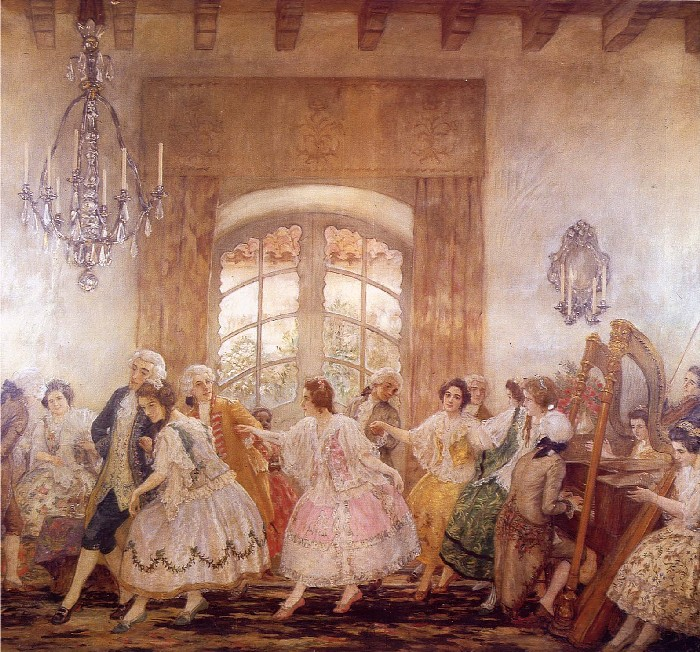
\includegraphics[scale=13.5]{/Users/hectorbahamonde/RU/Dissertation/Presentation/Resources/Baile_del_Santiago_antiguo}}\caption*{{\tiny `Baile del Santiago Antiguo.' Pedro Subercaseaux Err\'azuriz (1917).}}
		\label{fig:baile}
		\end{figure}
		
	\end{itemize}
\end{frame}





\miniframesoff

\begin{frame}\frametitle{Argument}
	\begin{itemize}
		
		\item[] The emergence of industrial elites imposed tight constrains on the way politics was run by agricultural elites.

		\begin{figure}[H]
		\vspace{1cm}
		\hspace{-9.2mm}
		%\centering
		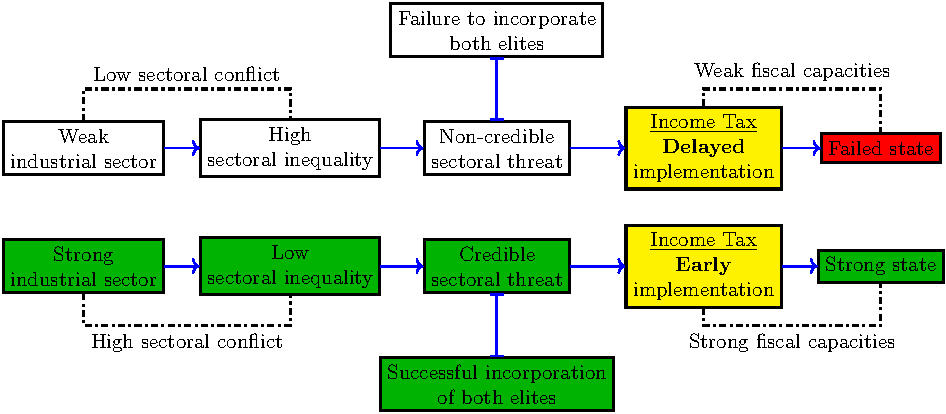
\includegraphics[scale=0.6]{/Users/hectorbahamonde/RU/Job_Market/causal_path_p1_strong}
		\end{figure}

	\end{itemize}
\end{frame}


\begin{frame}\frametitle{Argument}
	\begin{itemize}
		
		\item[] Industrial expansion reduced levels of inter-sectoral inequality, posing credible \hyperlink{credible_threats}{\beamerbutton{threats}}  to agricultural incumbents.

		\begin{figure}[H]
		\vspace{1cm}\hspace{-8mm}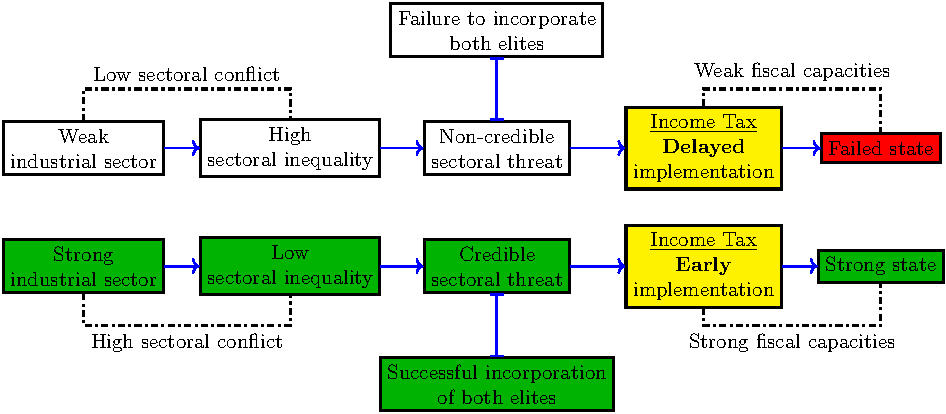
\includegraphics[scale=0.6]{/Users/hectorbahamonde/RU/Job_Market/causal_path_p1_strong}
		\end{figure}

	\end{itemize}
\end{frame}


\begin{frame}\frametitle{Argument}
	\begin{itemize}
		
		\item[] Given that both sectors were equally developed, both could get access to equally capable military resources.

		\begin{figure}[H]
		\vspace{1cm}\hspace{-8mm}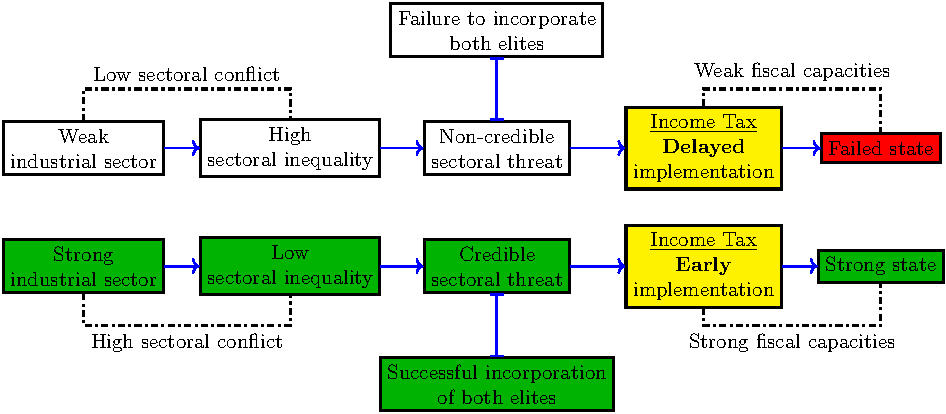
\includegraphics[scale=0.6]{/Users/hectorbahamonde/RU/Job_Market/causal_path_p1_strong}
		\end{figure}

	\end{itemize}
\end{frame}



\begin{frame}\frametitle{Argument}
	\begin{itemize}
		
		\item[] Also, industrial expansion required more infrastructure (public goods), such as roads and bridges. Hence industrial elites were more willing to pay for those via an income tax\tiny{---as opposed to import taxes.}

		\begin{figure}[H]
		\vspace{0.6cm}\hspace{-8mm}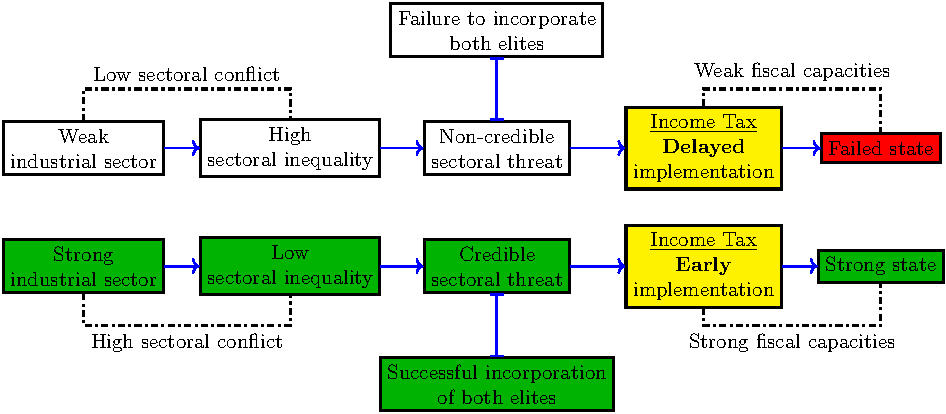
\includegraphics[scale=0.6]{/Users/hectorbahamonde/RU/Job_Market/causal_path_p1_strong}
		\end{figure}

	\end{itemize}
\end{frame}


\begin{frame}\frametitle{Argument}
	\begin{itemize}
		
		\item[] \scalerel*{
\includegraphics{/Users/hectorbahamonde/RU/Dissertation/Presentation/Resources/chilean-flag-large}}{B} I find that Chilean industrial elites accepted to be income taxed, while demanding political incorporation, and public infrastructure beneficial for industrial production.

		\begin{figure}[H]
		\vspace{.52cm}\hspace{-8mm}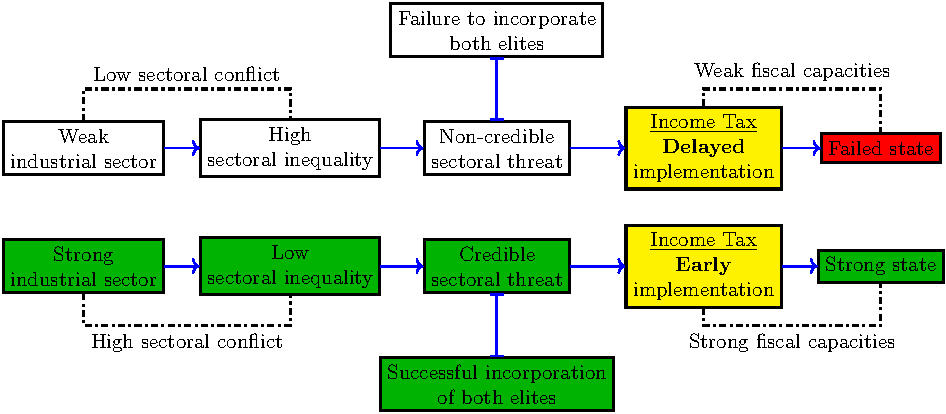
\includegraphics[scale=0.6]{/Users/hectorbahamonde/RU/Job_Market/causal_path_p1_strong}
		\end{figure}

	\end{itemize}
\end{frame}


\begin{frame}\frametitle{Argument}
	\begin{itemize}
		
		\item[] \scalerel*{
\includegraphics{/Users/hectorbahamonde/RU/Dissertation/Presentation/Resources/chilean-flag-large}}{B} As industrialists depended more on infrastructure implemented at the local level (roads, railroads and bridges), they preferred to shoulder a higher tax burden through progressive direct taxation.

		\begin{figure}[H]
		\vspace{.52cm}\hspace{-8mm}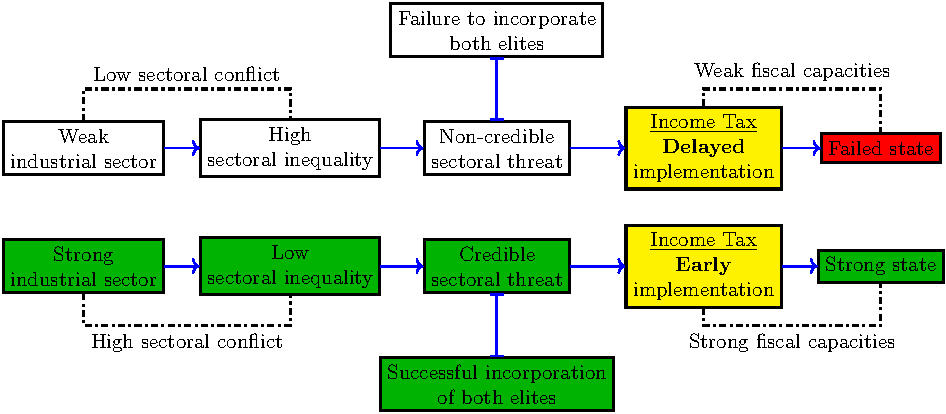
\includegraphics[scale=0.6]{/Users/hectorbahamonde/RU/Job_Market/causal_path_p1_strong}
		\end{figure}

	\end{itemize}
\end{frame}



\begin{frame}\frametitle{Argument}
	\begin{itemize}
		
		\item[] State presence became denser and complex, fostering state-making. Income {\bf taxation} was the main {\color{red}{\bf engine}} that promoted {\bf state-building}.


		\begin{figure}[H]
		\vspace{1cm}\hspace{-8mm}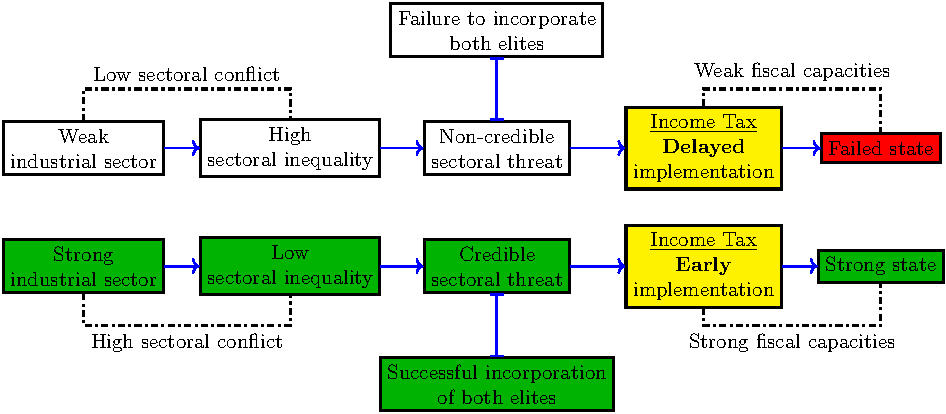
\includegraphics[scale=0.6]{/Users/hectorbahamonde/RU/Job_Market/causal_path_p1_strong}
		\end{figure}

	\end{itemize}
\end{frame}



\begin{frame}\frametitle{Argument}
	\begin{itemize}
		
		\item[] {\color{red}However}, a weak industrial sector engendered weak industrial elites unable to contest the institutional order. There was no need to make inter-sectoral alliances, {\bf {\color{red}delaying} the implementation of the income tax}.

		\begin{figure}[H]
		\vspace{0.5cm}\hspace{-8mm}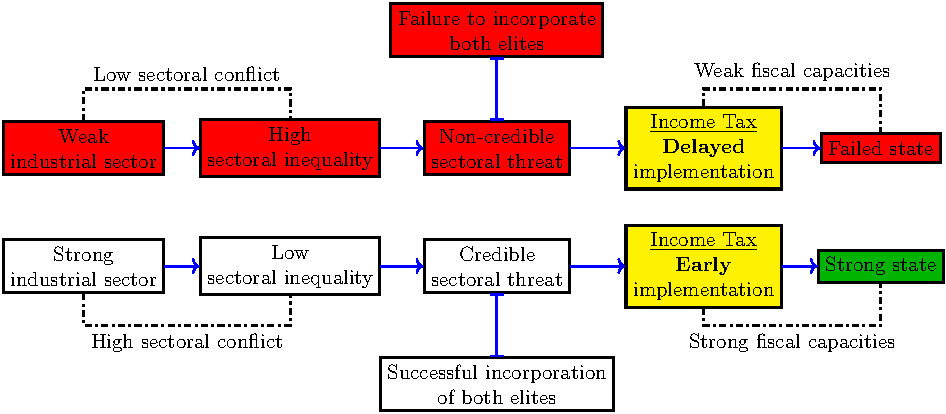
\includegraphics[scale=0.6]{/Users/hectorbahamonde/RU/Job_Market/causal_path_p1_failed}
		\end{figure}

	\end{itemize}
\end{frame}
\miniframeson

\subsection{Econometrics}


\begin{frame}\frametitle{When do countries implement the tax?}
	
	\begin{exampleblock}{`When' is a substantively important quantity of interest}
	An {\bf earlier} implementation situated the {\bf process} of implementing the law during the {\bf country's formative period}.
	\end{exampleblock}

	\begin{itemize}

		\item[] Early implementers were able to {\bf incorporate both elites} into the emergent national projects, {\bf crystallizing} a series of agreements that reflected both elites' preferences.


	\end{itemize}
\end{frame}


\miniframesoff
\begin{frame}\frametitle{When do countries implement the tax?}
	
	\begin{alertblock}{Late implementers?}
	Process was situated {\bf after} the country's formative period.
	\end{alertblock}

	\begin{itemize}
		\item While these countries eventually {\bf did impose the tax}, it was not product of an {\color{red}{\bf early domestic/endogenous}} process.

		\item {\bf No sectoral threat, no need for agreements}.\pause

		\item {\bf Guatemala}: it was exogenously imposed by the US-backed dictator Colonel Peralta, not necessarily reflecting the inter-sectoral domestic dynamics.

	\end{itemize}
\end{frame}




\miniframesoff
\begin{frame}\frametitle{Analyses}
	
	\begin{itemize}

		\item[Data] Proxy {\bf sectoral contestation} exploiting data on sectoral outputs (1900-2010) for a number of L.A. countries (MoxLaD).

		\item[Model] Duration models (Cox-Proportional \& Generalized Estimating Equations) to find out `who is to blame' for the {\color{black!30!green}early}/{\color{red}late} implementation of the income tax: \emph{Industrial or Agricultural elites?}

	\end{itemize}
\end{frame}



\miniframesoff

% \hspace{-1.1915cm} and scale=0.35
% for wide format

% Argentina
\begin{frame}[plain]
 \includegraphics[scale=0.35]{/Users/hectorbahamonde/RU/Dissertation/Papers/IncomeTaxAdoption/Argentina_Income_Tax.pdf}
\end{frame}


% Chile
\begin{frame}[plain]
 \includegraphics[scale=0.35]{/Users/hectorbahamonde/RU/Dissertation/Papers/IncomeTaxAdoption/Chile_Income_Tax.pdf}
\end{frame}


% Colombia
\begin{frame}[plain]
 \includegraphics[scale=0.35]{/Users/hectorbahamonde/RU/Dissertation/Papers/IncomeTaxAdoption/Colombia_Income_Tax.pdf}
\end{frame}

% Ecuador
\begin{frame}[plain]
 \includegraphics[scale=0.35]{/Users/hectorbahamonde/RU/Dissertation/Papers/IncomeTaxAdoption/Ecuador_Income_Tax.pdf}
\end{frame}

% Guatemala
\begin{frame}[plain]
 \includegraphics[scale=0.35]{/Users/hectorbahamonde/RU/Dissertation/Papers/IncomeTaxAdoption/Guatemala_Income_Tax.pdf}
\end{frame}


% Mexico
\begin{frame}[plain]
 \includegraphics[scale=0.35]{/Users/hectorbahamonde/RU/Dissertation/Papers/IncomeTaxAdoption/Mexico_Income_Tax.pdf}
\end{frame}


% Nicaragua
\begin{frame}[plain]
 \includegraphics[scale=0.35]{/Users/hectorbahamonde/RU/Dissertation/Papers/IncomeTaxAdoption/Nicaragua_Income_Tax.pdf}
\end{frame}


% Peru
\begin{frame}[plain]
 \includegraphics[scale=0.35]{/Users/hectorbahamonde/RU/Dissertation/Papers/IncomeTaxAdoption/Peru_Income_Tax.pdf}
\end{frame}


% Venezuela
\begin{frame}[plain]
 \includegraphics[scale=0.35]{/Users/hectorbahamonde/RU/Dissertation/Papers/IncomeTaxAdoption/Venezuela_Income_Tax.pdf}
\end{frame}


% 0
\begin{frame}[plain]
\scalebox{0.62}{

% \centering
\hspace{10mm}
\begin{tabular}{c||c|c|c|c|c}
 & \multicolumn{1}{c|}{Cox (1 lag)} & \multicolumn{1}{c|}{Cox (1 lag, ln)} & \multicolumn{1}{c|}{Logit GEE} & \multicolumn{1}{c|}{Conditional Logit (FE)} & \multicolumn{1}{c}{Spatial Dependence} \\
\hline
\hline

Manufacture Output$_{t-1}$       & 1.451$^{*}$    &               &             &              &         \\
                                 & (0.569)      &               &             &              &         \\
Agricultural Output$_{t-1}$      & -0.859       &               &             &              &         \\
                                 & (0.740)      &               &             &              &         \\
Total Population                 & -0.000$^{***}$ &               &             &              &         \\
                                 & (0.000)      &               &             &              &         \\
Manufacture Output$_{t-1}$ (ln)  &              & 1.279$^{\cdot}$ &             &              &         \\
                                 &              & (0.710)       &             &              &         \\
Agricultural Output$_{t-1}$ (ln) &              & -0.819        &             &              &         \\
                                 &              & (0.788)       &             &              &         \\
Total Population (ln)            &              & -0.844        & 0.065       & 1.012$^{*}$    & -0.842  \\
                                 &              & (0.531)       & (1.219)     & (0.405)      & (0.830) \\
Manufacture Output (ln)          &              &               & 1.543$^{***}$ & 0.970$^{***}$  & 1.277   \\
                                 &              &               & (0.333)     & (0.161)      & (1.036) \\
Agricultural Output (ln)         &              &               & -1.107$^{**}$ & -1.185$^{***}$ & -0.818  \\
                                 &              &               & (0.369)     & (0.292)      & (1.071) \\
\hline
AIC                              & 22.788       & 25.093        &             & 4135.812     & 25.091  \\
R$^2$                            & 0.021        & 0.013         &             & 0.392        & 0.013   \\
Max. R$^2$                       & 0.078        & 0.080         &             & 0.995        & 0.078   \\
Num. events                      & 9            & 9             &             & 570          & 9       \\
Num. obs.                        & 281          & 272           & 842         & 842          & 281     \\
Missings                         & 0            & 0             &             & 0            & 0       \\
PH test                          & 0.937        & 0.722         &             &              & 0.217   \\
Num. clust.                      &              &               & 9           &              &         \\
\hline
\multicolumn{6}{l}{\tiny{$^{***}p<0.001$, $^{**}p<0.01$, $^*p<0.05$, $^{\cdot}p<0.1$. Robust standard errors in all models}}
\end{tabular}
}
\end{frame}




% 00
\begin{frame}[plain]
\scalebox{0.62}{

%\centering
\hspace{10mm}
\begin{tabular}{c||c|c|c|c|c}
 & \multicolumn{1}{c|}{{\color{red}Cox (1 lag)}} & \multicolumn{1}{c|}{{\color{red}Cox (1 lag, ln)}} & \multicolumn{1}{c|}{{\color{red}Logit GEE}} & \multicolumn{1}{c|}{{\color{red}Conditional Logit (FE)}} & \multicolumn{1}{c}{{\color{red}Spatial Dependence}} \\
\hline
\hline

Manufacture Output$_{t-1}$       & 1.451$^{*}$    &               &             &              &         \\
                                 & (0.569)      &               &             &              &         \\
Agricultural Output$_{t-1}$      & -0.859       &               &             &              &         \\
                                 & (0.740)      &               &             &              &         \\
Total Population                 & -0.000$^{***}$ &               &             &              &         \\
                                 & (0.000)      &               &             &              &         \\
Manufacture Output$_{t-1}$ (ln)  &              & 1.279$^{\cdot}$ &             &              &         \\
                                 &              & (0.710)       &             &              &         \\
Agricultural Output$_{t-1}$ (ln) &              & -0.819        &             &              &         \\
                                 &              & (0.788)       &             &              &         \\
Total Population (ln)            &              & -0.844        & 0.065       & 1.012$^{*}$    & -0.842  \\
                                 &              & (0.531)       & (1.219)     & (0.405)      & (0.830) \\
Manufacture Output (ln)          &              &               & 1.543$^{***}$ & 0.970$^{***}$  & 1.277   \\
                                 &              &               & (0.333)     & (0.161)      & (1.036) \\
Agricultural Output (ln)         &              &               & -1.107$^{**}$ & -1.185$^{***}$ & -0.818  \\
                                 &              &               & (0.369)     & (0.292)      & (1.071) \\
\hline
AIC                              & 22.788       & 25.093        &             & 4135.812     & 25.091  \\
R$^2$                            & 0.021        & 0.013         &             & 0.392        & 0.013   \\
Max. R$^2$                       & 0.078        & 0.080         &             & 0.995        & 0.078   \\
Num. events                      & 9            & 9             &             & 570          & 9       \\
Num. obs.                        & 281          & 272           & 842         & 842          & 281     \\
Missings                         & 0            & 0             &             & 0            & 0       \\
PH test                          & 0.937        & 0.722         &             &              & 0.217   \\
Num. clust.                      &              &               & 9           &              &         \\
\hline
\multicolumn{6}{l}{\tiny{$^{***}p<0.001$, $^{**}p<0.01$, $^*p<0.05$, $^{\cdot}p<0.1$. Robust standard errors in all models}}
\end{tabular}
}
\end{frame}





% 1
\begin{frame}[plain]
\scalebox{0.62}{

%\centering
\hspace{10mm}
\begin{tabular}{c||c|c|c|c|c}
 & \multicolumn{1}{c|}{{\color{red}Cox (1 lag)}} & \multicolumn{1}{c|}{Cox (1 lag, ln)} & \multicolumn{1}{c|}{Logit GEE} & \multicolumn{1}{c|}{Conditional Logit (FE)} & \multicolumn{1}{c}{Spatial Dependence} \\
\hline
\hline

{\color{red}Manufacture Output$_{t-1}$}       & {\color{red}1.451$^{*}$}    &               &             &              &         \\
                                 & (0.569)      &               &             &              &         \\
{\color{red}Agricultural Output$_{t-1}$}      & {\color{red}-0.859}       &               &             &              &         \\
                                 & (0.740)      &               &             &              &         \\
Total Population                 & -0.000$^{***}$ &               &             &              &         \\
                                 & (0.000)      &               &             &              &         \\
Manufacture Output$_{t-1}$ (ln)  &              & 1.279$^{\cdot}$ &             &              &         \\
                                 &              & (0.710)       &             &              &         \\
Agricultural Output$_{t-1}$ (ln) &              & -0.819        &             &              &         \\
                                 &              & (0.788)       &             &              &         \\
Total Population (ln)            &              & -0.844        & 0.065       & 1.012$^{*}$    & -0.842  \\
                                 &              & (0.531)       & (1.219)     & (0.405)      & (0.830) \\
Manufacture Output (ln)          &              &               & 1.543$^{***}$ & 0.970$^{***}$  & 1.277   \\
                                 &              &               & (0.333)     & (0.161)      & (1.036) \\
Agricultural Output (ln)         &              &               & -1.107$^{**}$ & -1.185$^{***}$ & -0.818  \\
                                 &              &               & (0.369)     & (0.292)      & (1.071) \\
\hline
AIC                              & 22.788       & 25.093        &             & 4135.812     & 25.091  \\
R$^2$                            & 0.021        & 0.013         &             & 0.392        & 0.013   \\
Max. R$^2$                       & 0.078        & 0.080         &             & 0.995        & 0.078   \\
Num. events                      & 9            & 9             &             & 570          & 9       \\
Num. obs.                        & 281          & 272           & 842         & 842          & 281     \\
Missings                         & 0            & 0             &             & 0            & 0       \\
PH test                          & 0.937        & 0.722         &             &              & 0.217   \\
Num. clust.                      &              &               & 9           &              &         \\
\hline
\multicolumn{6}{l}{\tiny{$^{***}p<0.001$, $^{**}p<0.01$, $^*p<0.05$, $^{\cdot}p<0.1$. Robust standard errors in all models}}
\end{tabular}
}
\end{frame}



% 2
\begin{frame}[plain]
\scalebox{0.62}{

%\centering
\hspace{10mm}
\begin{tabular}{c||c|c|c|c|c}
 & \multicolumn{1}{c|}{Cox (1 lag)} & \multicolumn{1}{c|}{{\color{red}Cox (1 lag, ln)}} & \multicolumn{1}{c|}{Logit GEE} & \multicolumn{1}{c|}{Conditional Logit (FE)} & \multicolumn{1}{c}{Spatial Dependence} \\
\hline
\hline

Manufacture Output$_{t-1}$       & 1.451$^{*}$    &               &             &              &         \\
                                 & (0.569)      &               &             &              &         \\
Agricultural Output$_{t-1}$      & -0.859       &               &             &              &         \\
                                 & (0.740)      &               &             &              &         \\
Total Population                 & -0.000$^{***}$ &               &             &              &         \\
                                 & (0.000)      &               &             &              &         \\
{\color{red}Manufacture Output$_{t-1}$ (ln)}  &              & {\color{red}1.279$^{\cdot}$} &             &              &         \\
                                 &              & (0.710)       &             &              &         \\
{\color{red}Agricultural Output$_{t-1}$ (ln)} &              & {\color{red}-0.819}        &             &              &         \\
                                 &              & (0.788)       &             &              &         \\
Total Population (ln)            &              & -0.844        & 0.065       & 1.012$^{*}$    & -0.842  \\
                                 &              & (0.531)       & (1.219)     & (0.405)      & (0.830) \\
Manufacture Output (ln)          &              &               & 1.543$^{***}$ & 0.970$^{***}$  & 1.277   \\
                                 &              &               & (0.333)     & (0.161)      & (1.036) \\
Agricultural Output (ln)         &              &               & -1.107$^{**}$ & -1.185$^{***}$ & -0.818  \\
                                 &              &               & (0.369)     & (0.292)      & (1.071) \\
\hline
AIC                              & 22.788       & 25.093        &             & 4135.812     & 25.091  \\
R$^2$                            & 0.021        & 0.013         &             & 0.392        & 0.013   \\
Max. R$^2$                       & 0.078        & 0.080         &             & 0.995        & 0.078   \\
Num. events                      & 9            & 9             &             & 570          & 9       \\
Num. obs.                        & 281          & 272           & 842         & 842          & 281     \\
Missings                         & 0            & 0             &             & 0            & 0       \\
PH test                          & 0.937        & 0.722         &             &              & 0.217   \\
Num. clust.                      &              &               & 9           &              &         \\
\hline
\multicolumn{6}{l}{\tiny{$^{***}p<0.001$, $^{**}p<0.01$, $^*p<0.05$, $^{\cdot}p<0.1$. Robust standard errors in all models}}
\end{tabular}
}
\end{frame}


% 3
\begin{frame}[plain]
\scalebox{0.62}{

%\centering
\hspace{10mm}
\begin{tabular}{c||c|c|c|c|c}
 & \multicolumn{1}{c|}{Cox (1 lag)} & \multicolumn{1}{c|}{Cox (1 lag, ln)} & \multicolumn{1}{c|}{{\color{red}Logit GEE}} & \multicolumn{1}{c|}{Conditional Logit (FE)} & \multicolumn{1}{c}{Spatial Dependence} \\
\hline
\hline

Manufacture Output$_{t-1}$       & 1.451$^{*}$    &               &             &              &         \\
                                 & (0.569)      &               &             &              &         \\
Agricultural Output$_{t-1}$      & -0.859       &               &             &              &         \\
                                 & (0.740)      &               &             &              &         \\
Total Population                 & -0.000$^{***}$ &               &             &              &         \\
                                 & (0.000)      &               &             &              &         \\
Manufacture Output$_{t-1}$ (ln)  &              & 1.279$^{\cdot}$ &             &              &         \\
                                 &              & (0.710)       &             &              &         \\
Agricultural Output$_{t-1}$ (ln) &              & -0.819        &             &              &         \\
                                 &              & (0.788)       &             &              &         \\
Total Population (ln)            &              & -0.844        & 0.065       & 1.012$^{*}$    & -0.842  \\
                                 &              & (0.531)       & (1.219)     & (0.405)      & (0.830) \\
{\color{red}Manufacture Output (ln)}          &              &               & {\color{red}1.543$^{***}$} & 0.970$^{***}$  & 1.277   \\
                                 &              &               & (0.333)     & (0.161)      & (1.036) \\
{\color{red}Agricultural Output (ln)}         &              &               & {\color{red}-1.107$^{**}$} & -1.185$^{***}$ & -0.818  \\
                                 &              &               & (0.369)     & (0.292)      & (1.071) \\
\hline
AIC                              & 22.788       & 25.093        &             & 4135.812     & 25.091  \\
R$^2$                            & 0.021        & 0.013         &             & 0.392        & 0.013   \\
Max. R$^2$                       & 0.078        & 0.080         &             & 0.995        & 0.078   \\
Num. events                      & 9            & 9             &             & 570          & 9       \\
Num. obs.                        & 281          & 272           & 842         & 842          & 281     \\
Missings                         & 0            & 0             &             & 0            & 0       \\
PH test                          & 0.937        & 0.722         &             &              & 0.217   \\
Num. clust.                      &              &               & 9           &              &         \\
\hline
\multicolumn{6}{l}{\tiny{$^{***}p<0.001$, $^{**}p<0.01$, $^*p<0.05$, $^{\cdot}p<0.1$. Robust standard errors in all models}}
\end{tabular}
}
\end{frame}


% 4
\begin{frame}[plain]
\scalebox{0.62}{

%\centering
\hspace{10mm}
\begin{tabular}{c||c|c|c|c|c}
 & \multicolumn{1}{c|}{Cox (1 lag)} & \multicolumn{1}{c|}{Cox (1 lag, ln)} & \multicolumn{1}{c|}{Logit GEE} & \multicolumn{1}{c|}{{\color{red}Conditional Logit (FE)}} & \multicolumn{1}{c}{Spatial Dependence} \\
\hline
\hline

Manufacture Output$_{t-1}$       & 1.451$^{*}$    &               &             &              &         \\
                                 & (0.569)      &               &             &              &         \\
Agricultural Output$_{t-1}$      & -0.859       &               &             &              &         \\
                                 & (0.740)      &               &             &              &         \\
Total Population                 & -0.000$^{***}$ &               &             &              &         \\
                                 & (0.000)      &               &             &              &         \\
Manufacture Output$_{t-1}$ (ln)  &              & 1.279$^{\cdot}$ &             &              &         \\
                                 &              & (0.710)       &             &              &         \\
Agricultural Output$_{t-1}$ (ln) &              & -0.819        &             &              &         \\
                                 &              & (0.788)       &             &              &         \\
Total Population (ln)            &              & -0.844        & 0.065       & 1.012$^{*}$    & -0.842  \\
                                 &              & (0.531)       & (1.219)     & (0.405)      & (0.830) \\
{\color{red}Manufacture Output (ln)}          &              &               & 1.543$^{***}$ & {\color{red}0.970$^{***}$}  & 1.277   \\
                                 &              &               & (0.333)     & (0.161)      & (1.036) \\
{\color{red}Agricultural Output (ln)}         &              &               & -1.107$^{**}$ & {\color{red}-1.185$^{***}$} & -0.818  \\
                                 &              &               & (0.369)     & (0.292)      & (1.071) \\
\hline
AIC                              & 22.788       & 25.093        &             & 4135.812     & 25.091  \\
R$^2$                            & 0.021        & 0.013         &             & 0.392        & 0.013   \\
Max. R$^2$                       & 0.078        & 0.080         &             & 0.995        & 0.078   \\
Num. events                      & 9            & 9             &             & 570          & 9       \\
Num. obs.                        & 281          & 272           & 842         & 842          & 281     \\
Missings                         & 0            & 0             &             & 0            & 0       \\
PH test                          & 0.937        & 0.722         &             &              & 0.217   \\
Num. clust.                      &              &               & 9           &              &         \\
\hline
\multicolumn{6}{l}{\tiny{$^{***}p<0.001$, $^{**}p<0.01$, $^*p<0.05$, $^{\cdot}p<0.1$. Robust standard errors in all models}}
\end{tabular}
}
\end{frame}


% 5
\begin{frame}[plain]
\scalebox{0.62}{

%\centering
\hspace{10mm}
\begin{tabular}{c||c|c|c|c|c}
 & \multicolumn{1}{c|}{Cox (1 lag)} & \multicolumn{1}{c|}{Cox (1 lag, ln)} & \multicolumn{1}{c|}{Logit GEE} & \multicolumn{1}{c|}{Conditional Logit (FE)} & \multicolumn{1}{c}{{\color{red}Spatial Dependence}} \\
\hline
\hline

Manufacture Output$_{t-1}$       & 1.451$^{*}$    &               &             &              &         \\
                                 & (0.569)      &               &             &              &         \\
Agricultural Output$_{t-1}$      & -0.859       &               &             &              &         \\
                                 & (0.740)      &               &             &              &         \\
Total Population                 & -0.000$^{***}$ &               &             &              &         \\
                                 & (0.000)      &               &             &              &         \\
Manufacture Output$_{t-1}$ (ln)  &              & 1.279$^{\cdot}$ &             &              &         \\
                                 &              & (0.710)       &             &              &         \\
Agricultural Output$_{t-1}$ (ln) &              & -0.819        &             &              &         \\
                                 &              & (0.788)       &             &              &         \\
Total Population (ln)            &              & -0.844        & 0.065       & 1.012$^{*}$    & -0.842  \\
                                 &              & (0.531)       & (1.219)     & (0.405)      & (0.830) \\
{\color{red}Manufacture Output (ln)}          &              &               & 1.543$^{***}$ & 0.970$^{***}$  & {\color{red}1.277}   \\
                                 &              &               & (0.333)     & (0.161)      & (1.036) \\
{\color{red}Agricultural Output (ln)}         &              &               & -1.107$^{**}$ & -1.185$^{***}$ & {\color{red}-0.818}  \\
                                 &              &               & (0.369)     & (0.292)      & (1.071) \\
\hline
AIC                              & 22.788       & 25.093        &             & 4135.812     & 25.091  \\
R$^2$                            & 0.021        & 0.013         &             & 0.392        & 0.013   \\
Max. R$^2$                       & 0.078        & 0.080         &             & 0.995        & 0.078   \\
Num. events                      & 9            & 9             &             & 570          & 9       \\
Num. obs.                        & 281          & 272           & 842         & 842          & 281     \\
Missings                         & 0            & 0             &             & 0            & 0       \\
PH test                          & 0.937        & 0.722         &             &              & 0.217   \\
Num. clust.                      &              &               & 9           &              &         \\
\hline
\multicolumn{6}{l}{\tiny{$^{***}p<0.001$, $^{**}p<0.01$, $^*p<0.05$, $^{\cdot}p<0.1$. Robust standard errors in all models}}
\end{tabular}
}
\end{frame}


\miniframesoff
\begin{frame}%\frametitle{}

\begin{itemize}
	\item[] {\bf Simulated sectoral hazard rates} of implementing the income tax law.
	\item[] HR: probability that a case will fail at time $t$.
\end{itemize}
	
	\begin{figure}[H]
	\hspace{-17mm}
	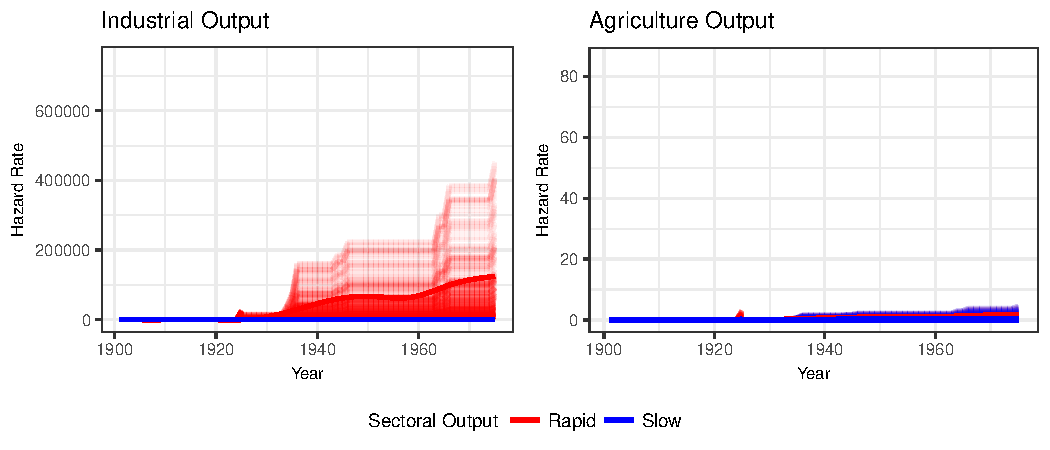
\includegraphics[width=1.0\textwidth]{/Users/hectorbahamonde/RU/Dissertation/Presentation/Resources/simulation:plots-1.pdf}
	\end{figure}
	
\end{frame}



\miniframesoff
\begin{frame}[plain, c]
\begin{center}
\Large \href{https://github.com/hbahamonde/Earthquake_Paper/raw/master/Bahamonde_Earthquake_Paper.pdf}{\input{/Users/hectorbahamonde/RU/Dissertation/Papers/Earthquake_Paper/title.txt}\unskip}
\end{center}
\end{frame}
\miniframeson


% p.3
\section{State Capacities}

% research question 2
\miniframesoff
\begin{frame}[c]\frametitle{Research Question}
\begin{center}
\huge{What have been the {\bf effects} of fiscal expansion on state capacities overtime, and how can they be {\bf measured}?}\pause
\\
\vspace{1.3cm}
\large{Use a novel hand-collected longitudinal {\bf dataset on earthquakes death tolls} to proxy the \emph{capacity} of the state to enforce building codes at the subnational level.}\pause\;{\bf State capacities increase overtime upon the implementation of the income tax}.
\end{center}
\end{frame}

% motivation
\subsection{Earthquakes and State Capacities}




\subsection{Motivation}
\miniframeson




\begin{frame}
	\begin{itemize}
		\item[] The first section helps us to understand \emph{when} countries implement the income tax, and \emph{why} timing is relevant.\pause\; However, the first section doesn't link income taxation with \emph{actual} state capacities.\pause%\; Historians and fiscal sociologists provide some answers, but this relationship in the Latin American political economies has been overlooked.\pause\; \emph{{\bf Did the expansion of the fiscal system improve state capacities overtime in Latin America?}}\pause

		\item[\tiny{Mechanism}] Beyond `\emph{War makes states and states make war}.' Domestic-based mechanism.

		\item[\tiny{Measurement}] \emph{How} can we {\bf measure} the effects of income taxation on state of capacities overtime?

\pause\dotfill

	\item[{\color{red}$\star$}] {\bf Historians} and {\bf fiscal sociologists} provide some answers, but the {\bf {\color{red}sectoral approach}} on the relationship between {\bf income taxation} and {\bf state capacities} has been overlooked in the Latin American context.\pause

	\item[{\color{red}$\star$}] Most {\bf theories} of state-building in comparative politics are historical. Yet, most {\bf measurements} capture \emph{contemporaneous} levels of state-capacities. {\color{red}Earthquake death tolls}.
	\end{itemize}

\end{frame}






\miniframesoff
\begin{frame}\frametitle{Why Earthquakes?}

\begin{itemize}
	\item[] Earthquakes are {\bf exogenous} to regime type, levels of political/economic development, and other sources of variation.
\end{itemize}

	\vspace{-0.2cm}
		
		\begin{figure}[H]
		\hspace{-7mm}\frame{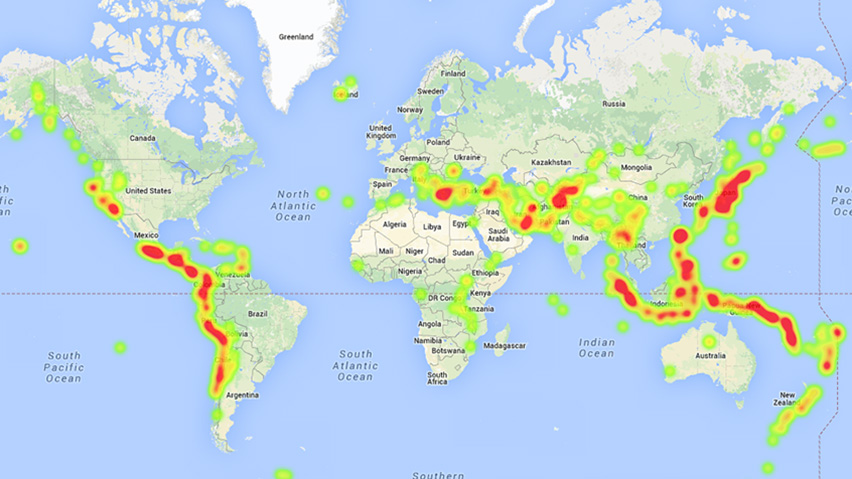
\includegraphics[scale=0.33]{/Users/hectorbahamonde/RU/Dissertation/Presentation/Resources/quake_map.jpg}}
		\end{figure}
	
\end{frame}









%\miniframesoff
%\begin{frame}\frametitle{Why Earthquakes?}
%
%\begin{itemize}
%	\item[] Importantly, enforcing these codes requires agreements with the subnational level. Subnational elites might not be interested in applying norms designed in the capital.
%\end{itemize}
%
%		
%		\begin{figure}[H]
%		%\vspace{20mm}\hspace{-30mm}
%		\frame{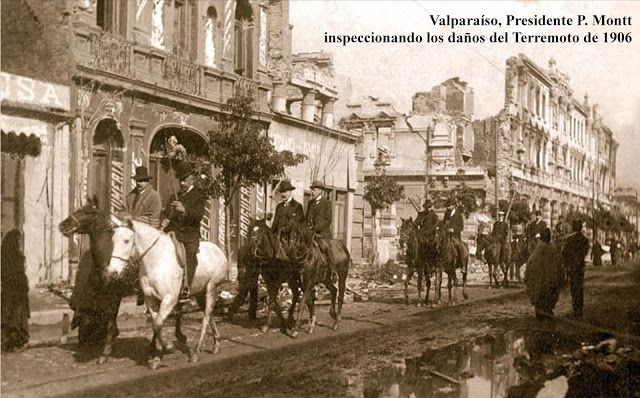
\includegraphics[scale=0.39]{/Users/hectorbahamonde/RU/Dissertation/Presentation/Resources/Montt_quake}}
%		\end{figure}
%	
%
%\end{frame}


\subsection{Argument}

\miniframeson
\begin{frame}\frametitle{Thinking Subnationally}
	\begin{itemize}
		
		\item[] Since death tolls are a function of how well/bad building codes are enforced by the state throughout the {\bf territory}, adopting a {\bf subnational} approach seems more appropriate.

		\begin{figure}[H]
		%\vspace{0.3cm}
		\hspace{-8mm}\includegraphics[scale=0.7]{/Users/hectorbahamonde/RU/Dissertation/Papers/Earthquake_Paper/causal_path}
		\end{figure}

	\end{itemize}
\end{frame}

\miniframesoff
\begin{frame}\frametitle{Argument}
	\begin{itemize}
		
		\item[] Argue that higher levels of subnational and national sectoral contestation fostered state-capacities overtime.


		\begin{figure}[H]
		\vspace{5mm}\hspace{-8mm}\includegraphics[scale=0.7]{/Users/hectorbahamonde/RU/Dissertation/Papers/Earthquake_Paper/causal_path}
		\end{figure}

	\end{itemize}
\end{frame}



\miniframesoff
\begin{frame}\frametitle{Argument}
	\begin{itemize}
		
		\item[] \underline{{\bf Conceptualizing contestation}}: {\bf {\color{red}regional} industrial expansion} contesting {\bf agricultural {\color{red}national}} economic hegemony.


		\begin{figure}[H]
		\vspace{5mm}\hspace{-8mm}\includegraphics[scale=0.7]{/Users/hectorbahamonde/RU/Dissertation/Papers/Earthquake_Paper/causal_path}
		\end{figure}

	\end{itemize}
\end{frame}




\miniframesoff
\begin{frame}\frametitle{{\large Incorporation of Subnational Elites into the National State-Making Project}}

	\begin{exampleblock}{Subnational/National Connection}{
		Higher levels of subnational industrial expansion posed \hyperlink{credible_threats}{\beamerbutton{credible threats}} to the landed elites at the national level. \pause Agreements were required to avoid military conflicts\pause. Contingent on the delivery of subnational public goods, local elites agreed to cooperate with the central level, and comply with the {\bf income tax}.}
	\end{exampleblock}

\end{frame}







\miniframesoff
\begin{frame}\frametitle{Argument}

	\begin{exampleblock}{Increasing the density of state presence overtime}{
	\scalerel*{
\includegraphics{/Users/hectorbahamonde/RU/Dissertation/Presentation/Resources/chilean-flag-large}}{B}  The implementation of the income tax improved state-capacities over time. \pause Activities such as {\bf deployment} of tax collectors to inspect accounting books and to supervise monetary transfers between individuals increased the {\color{red}density of state presence overtime.}}
	\end{exampleblock}


\end{frame}


\subsection{Econometrics}


\miniframeson
\begin{frame}\frametitle{The Theory Should Pass Two Tests}
	
	\begin{enumerate}
		\item The state should have higher capacities (i.e. \emph{lower death tolls}) when subnationally contested.

		\item Implementation of the income tax should produce higher state-capacities (i.e. \emph{lower death tolls}) overtime.
	\end{enumerate}

\end{frame}



\miniframesoff
\begin{frame}\frametitle{Analyses}
	
	\begin{itemize}
		\item[Data] Subnational and national Chilean data (1907 to 2012).
				
				\begin{itemize}
					\item[{\tiny National}] Sectoral outputs. \hyperlink{proportion_variable}{\beamerbutton{Just like before}}
					
					\item[{\tiny Subnational}] NOAA database as a starting point.\pause

					\item[{\tiny Subnational}] Using archival data (historical newspapers and censuses 1907 onwards), I complemented these data with:

						\begin{enumerate}
							\item Municipal population (to weight death tolls).
							\item Municipal main economic sector.
						\end{enumerate}
				
				\end{itemize} 

		\pause \item[Model] {\color{blue}Bayesian Hierarchical Poisson model with year fixed-effects} to account for the count of deaths. \hyperlink{jags_code}{\beamerbutton{Jags Code}}
	\end{itemize}

\end{frame}



\miniframesoff
\begin{frame}[plain]%\frametitle{Analyses}

		\begin{figure}[H]
		\vspace{4mm}
		\hspace{-7.5mm}\includegraphics[scale=0.7]{/Users/hectorbahamonde/RU/Dissertation/Papers/Earthquake_Paper/figure/earthquake:ts:plot:chile-1.pdf}
		\end{figure}

\end{frame}


\miniframesoff
\begin{frame}[plain]%\frametitle{Analyses}

		\begin{figure}[H]
		\vspace{-5mm}
		%\hspace{-10mm}
		\includegraphics[scale=0.27]{/Users/hectorbahamonde/RU/Dissertation/Papers/Earthquake_Paper/Resources/chile_quake_map.jpeg}
		\end{figure}

\end{frame}



\miniframesoff
\begin{frame}\frametitle{{\large Estimating Effects of Subnational Contestation on Death Tolls}}

\begin{equation*}
  \begin{array}{ll}
\text{Deaths} & \;\sim\; \text{Poisson}(\lambda_{i}) \hspace{4.1cm}\hyperlink{death_count_plot}{\beamerbutton{Distribution of Deaths}}
\vspace{5mm}
\\
log(\lambda_{i})  &= 
\;\mu + 
\beta_{1_j}\text{Proportion}_{i} + 
\beta_{2_j}\text{Magnitude}^2_{i} +
\beta_{3}\text{Latitude}_{i} + \\
& \beta_{4}\text{Longitude}_{i} +
\beta_{5}\text{Population}_{i} +
\beta_{6}\text{Urban}_{i} + 
\beta_{7_t}\text{Year}_{i}
  \end{array}
\end{equation*}


where,

\begin{equation*} 
\begin{split}
i_{1,...I} & \; \text{where} \; \text{I}=91\;\text{earthquakes}\\
j_{1,...J} & \; \text{where} \; \text{J}=3\;\text{sectors (agr, ind, mixed)}\\
t_{1,...T} & \; \text{where} \; \text{T}=59\;\text{years.}
\end{split}
\end{equation*}


\begin{itemize}
	\item[] 4 chains, 200K iterations, burn-in of 5000.
	\item[] \vspace{5mm}
	\hspace{-1cm} 
	\hyperlink{density_plot_sectoral}{\beamerbutton{Densities}} \hyperlink{trace_plot_sectoral}{\beamerbutton{Trace plots}} \hyperlink{model_fit}{\beamerbutton{Model fit}} \hyperlink{table_sectoral}{\beamerbutton{Table}}  \href{https://github.com/hbahamonde/Earthquake_Paper/raw/master/Bahamonde_Earthquake_Paper_Diagnostic_Plots_Sectoral_Competition.pdf}{\beamerbutton{Download detailed diagnostics plots}} \hyperlink{proportion_variable}{\beamerbutton{Proportion}}
\end{itemize}
\end{frame}




\miniframesoff
\begin{frame}\frametitle{{\large Estimating Effects of Subnational Contestation on Death Tolls}}

\begin{equation*}
  \begin{array}{ll}
\text{Deaths} & \;\sim\; \text{Poisson}(\lambda_{i}) \hspace{4.1cm}\hyperlink{death_count_plot}{\beamerbutton{Distribution of Deaths}}
\vspace{5mm}
\\
log(\lambda_{i})  &= 
\;\mu + 
\beta_{1_j}\text{{\color{red}Proportion}}_{i} + 
\beta_{2_j}\text{Magnitude}^2_{i} +
\beta_{3}\text{Latitude}_{i} + \\
& \beta_{4}\text{Longitude}_{i} +
\beta_{5}\text{Population}_{i} +
\beta_{6}\text{Urban}_{i} + 
\beta_{7_t}\text{Year}_{i}
  \end{array}
\end{equation*}


where,

\begin{equation*} 
\begin{split}
i_{1,...I} & \; \text{where} \; \text{I}=91\;\text{earthquakes}\\
j_{1,...J} & \; \text{where} \; \text{J}=3\;\text{sectors (agr, ind, mixed)}\\
t_{1,...T} & \; \text{where} \; \text{T}=59\;\text{years.}
\end{split}
\end{equation*}


\begin{itemize}
	\item[] 4 chains, 200K iterations, burn-in of 5000.
	\item[] \vspace{5mm}
	\hspace{-1cm} 
	\hyperlink{density_plot_sectoral}{\beamerbutton{Densities}} \hyperlink{trace_plot_sectoral}{\beamerbutton{Trace plots}} \hyperlink{model_fit}{\beamerbutton{Model fit}} \hyperlink{table_sectoral}{\beamerbutton{Table}}  \href{https://github.com/hbahamonde/Earthquake_Paper/raw/master/Bahamonde_Earthquake_Paper_Diagnostic_Plots_Sectoral_Competition.pdf}{\beamerbutton{Download detailed diagnostics plots}} \hyperlink{proportion_variable}{\beamerbutton{Proportion}}
\end{itemize}
\end{frame}



\miniframesoff
\begin{frame}\frametitle{{\large Estimating Effects of Subnational Contestation on Death Tolls}}

\begin{equation*}
  \begin{array}{ll}
\text{Deaths} & \;\sim\; \text{Poisson}(\lambda_{i}) \hspace{4.1cm}\hyperlink{death_count_plot}{\beamerbutton{Distribution of Deaths}}
\vspace{5mm}
\\
log(\lambda_{i})  &= 
\;\mu + 
\beta_{1_\text{{\color{red}\emph{j}}}}\text{Proportion}_{i} + 
\beta_{2_j}\text{Magnitude}^2_{i} +
\beta_{3}\text{Latitude}_{i} + \\
& \beta_{4}\text{Longitude}_{i} +
\beta_{5}\text{Population}_{i} +
\beta_{6}\text{Urban}_{i} + 
\beta_{7_t}\text{Year}_{i}
  \end{array}
\end{equation*}


where,

\begin{equation*} 
\begin{split}
i_{1,...I} & \; \text{where} \; \text{I}=91\;\text{earthquakes}\\
j_{1,...\text{{\color{red}J}}} & \; \text{where} \; \text{{\color{red}J}}=3\;\text{{\color{red}sectors (agr, ind, mixed)}}\\
t_{1,...T} & \; \text{where} \; \text{T}=59\;\text{years.}
\end{split}
\end{equation*}


\begin{itemize}
	\item[] 4 chains, 200K iterations, burn-in of 5000.
	\item[] \vspace{5mm}
	\hspace{-1cm} 
	\hyperlink{density_plot_sectoral}{\beamerbutton{Densities}} \hyperlink{trace_plot_sectoral}{\beamerbutton{Trace plots}} \hyperlink{model_fit}{\beamerbutton{Model fit}} \hyperlink{table_sectoral}{\beamerbutton{Table}}  \href{https://github.com/hbahamonde/Earthquake_Paper/raw/master/Bahamonde_Earthquake_Paper_Diagnostic_Plots_Sectoral_Competition.pdf}{\beamerbutton{Download detailed diagnostics plots}} \hyperlink{proportion_variable}{\beamerbutton{Proportion}}
\end{itemize}

\end{frame}



\begin{frame}\frametitle{{\large Estimating Effects of Subnational Contestation on Death Tolls}}
 %\hspace{-1.16cm}
 \centering\includegraphics[scale=0.75]{/Users/hectorbahamonde/RU/Dissertation/Papers/Earthquake_Paper/figure/sectoral:model:plot:run-1.pdf}
\end{frame}




\miniframesoff
\begin{frame}\frametitle{{\large Estimating Effects of Income Taxation on Death Tolls Overtime}}

\begin{equation*}
  \begin{array}{ll}
\text{Deaths} & \;\sim\; \text{Poisson}(\lambda_{i}) \hspace{4.1cm}\hyperlink{death_count_plot}{\beamerbutton{Distribution of Deaths}}
\vspace{5mm}
\\
log(\lambda_{i})  &= 
\;\mu + 
\beta_{1}\text{Income Tax}_{i} + 
\beta_{2}\text{Magnitude}^2_{i} +
\beta_{3}\text{Latitude}_{i} + \\
&\beta_{4}\text{Longitude}_{i} +
\beta_{5}\text{Population}_{i} +
\beta_{6}\text{Urban}_{i} + 
\beta_{7_t}\text{Year}_{i}
  \end{array}
\end{equation*}


where,

\begin{equation*} 
\begin{split}
i_{1,...I} & \; \text{where} \; \text{I}=91\;\text{earthquakes}\\
t_{1,...T} & \; \text{where} \; \text{T}=59\;\text{years.}
\end{split}
\end{equation*}


\begin{itemize}
	\item[] 4 chains, 200K iterations, burn-in of 5000.
	\item[] \vspace{5mm}
	\hspace{-1cm} 
	\hyperlink{density_plot_tax}{\beamerbutton{Densities}} \hyperlink{trace_plot_tax}{\beamerbutton{Trace plots}} \hyperlink{model_fit}{\beamerbutton{Model fit}} \hyperlink{table_tax}{\beamerbutton{Table}}  \href{https://github.com/hbahamonde/Earthquake_Paper/raw/master/Bahamonde_Earthquake_Paper_Diagnostic_Plots_Income_Tax_Model.pdf}{\beamerbutton{Download detailed diagnostics plots}}
\end{itemize}
\end{frame}


\miniframesoff
\begin{frame}\frametitle{{\large Estimating Effects of Income Taxation on Death Tolls Overtime}}

\begin{equation*}
  \begin{array}{ll}
\text{Deaths} & \;\sim\; \text{Poisson}(\lambda_{i}) \hspace{4.1cm}\hyperlink{death_count_plot}{\beamerbutton{Distribution of Deaths}}
\vspace{5mm}
\\
log(\lambda_{i})  &= 
\;\mu + 
\beta_{1}\text{{\color{red}Income Tax}}_{i} + 
\beta_{2}\text{Magnitude}^2_{i} +
\beta_{3}\text{Latitude}_{i} + \\
&\beta_{4}\text{Longitude}_{i} +
\beta_{5}\text{Population}_{i} +
\beta_{6}\text{Urban}_{i} + 
\beta_{7_t}\text{Year}_{i}
  \end{array}
\end{equation*}


where,

\begin{equation*} 
\begin{split}
i_{1,...I} & \; \text{where} \; \text{I}=91\;\text{earthquakes}\\
t_{1,...T} & \; \text{where} \; \text{T}=59\;\text{years.}
\end{split}
\end{equation*}


\begin{itemize}
	\item[] 4 chains, 200K iterations, burn-in of 5000.
	\item[] \vspace{5mm}
	\hspace{-1cm} 
	\hyperlink{density_plot_tax}{\beamerbutton{Densities}} \hyperlink{trace_plot_tax}{\beamerbutton{Trace plots}} \hyperlink{model_fit}{\beamerbutton{Model fit}} \hyperlink{table_tax}{\beamerbutton{Table}}  \href{https://github.com/hbahamonde/Earthquake_Paper/raw/master/Bahamonde_Earthquake_Paper_Diagnostic_Plots_Income_Tax_Model.pdf}{\beamerbutton{Download detailed diagnostics plots}}
\end{itemize}
\end{frame}




\begin{frame}\frametitle{{\large Estimating Effects of Income Taxation on Death Tolls Overtime}}
 %\hspace{-1.16cm}
  \centering\includegraphics[scale=0.75]{/Users/hectorbahamonde/RU/Dissertation/Papers/Earthquake_Paper/figure/income:tax:model:plot:run-1.pdf}
\end{frame}



\section{Conclusion}
\miniframeson

\subsection{Summary}


% Summary frame
\miniframesoff
\begin{frame}[plain,c]
	\begin{center}
	\vspace{5mm}
	\Huge Summary
	\end{center}
\end{frame}

\subsection{P1}


%% p1
\miniframeson
\begin{frame}\frametitle{Income Tax Adoption}

\begin{itemize}
\item[] The emergence of the industrial sector \emph{accelerated the implementation of the income tax}. The tax was not important for the new revenue it collected, but because it forced inter-elite compromises that were beneficial for sate-\emph{making}.
\end{itemize}

	\begin{figure}[H]
	%\hspace{-17mm}
	\centering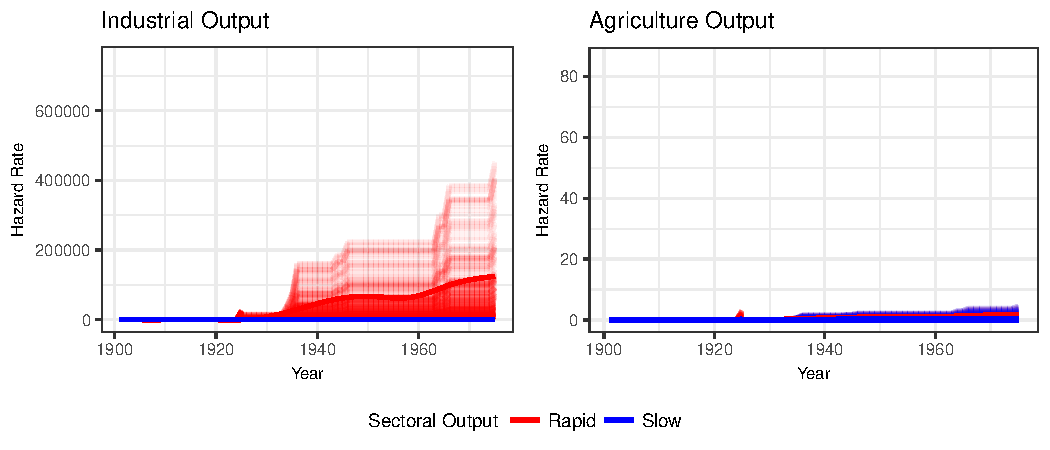
\includegraphics[width=1.0\textwidth]{/Users/hectorbahamonde/RU/Dissertation/Presentation/Resources/simulation:plots-1.pdf}
	\end{figure}
\end{frame}


\subsection{P2}


%% p2	
%\miniframesoff
\begin{frame}\frametitle{Balanced Growth and Income Tax}

\begin{itemize}
	\item[] When the income tax was implemented under \emph{contested} scenarios,\footnotemark elite incorporation changed the institutional order, fostering long-term economic growth.
\end{itemize}

	\begin{figure}[H]
	\vspace{-5mm}
	\centering\includegraphics[scale=0.4]{/Users/hectorbahamonde/RU/Dissertation/Papers/NegativeLink/Chile_StructuralBreak.pdf}	
	\end{figure}
\footnotetext[1]{{\tiny When sectoral cleavage was \emph{strong}, i.e. (1) cointegration and (2) reversal / Granger tests.}} 
\end{frame}

\subsection{P3}


%% p3:a
%\miniframesoff
\begin{frame}\frametitle{Earthquakes, Income Tax and State Capacities}
\begin{itemize}
	\item[] Subnational sources of sectoral contestation increased state-capacities.
\end{itemize}
	
	\begin{figure}[H]
	%\hspace{-17mm}
	\centering\includegraphics[scale=0.75]{/Users/hectorbahamonde/RU/Dissertation/Papers/Earthquake_Paper/figure/sectoral:model:plot:run-1.pdf}
	\end{figure}
\end{frame}

%% p3:b
\miniframesoff
\begin{frame}\frametitle{Earthquakes, Income Tax and State Capacities}
\begin{itemize}
	\item[] The implementation of the income tax was a state-\emph{making} institution, increasing state-capacities overtime.
\end{itemize}
	
	\begin{figure}[H]
	%\hspace{-17mm}
	\centering\includegraphics[scale=0.75]{/Users/hectorbahamonde/RU/Dissertation/Papers/Earthquake_Paper/figure/income:tax:model:plot:run-1.pdf}
	\end{figure}
\end{frame}




\miniframeson
\subsection{Future Research}


\begin{frame}\frametitle{What's Ahead}

\begin{itemize}
	\item I will collect more earthquake data for more countries.
	\item I will add more historical evidence, and try to see what's beyond the Chilean case.
	\item Others.
	\end{itemize}
\end{frame}





%%%%%%%%%%%%%%%%%%%%%%%%%%%%%%%%%%%%%%%%%%%%%%%%%%%%%%%%%%%%%%%%%%%%%%%%%%
%%%%%%%%%%%%%%%%%%%%%%%%%%%%%%%%%%%%%%%%%%%%%%%%%%%%%%%%%%%%%%%%%%%%%%%%%%
%%%%%%%%%%%%%%%%%%%%%%%%%%%%%%%%%%%%%%%%%%%%%%%%%%%%%%%%%%%%%%%%%%%%%%%%%%
%%%%%%%%%%%%%%%%%%%%%%%%%%%%%%%%%%%%%%%%%%%%%%%%%%%%%%%%%%%%%%%%%%%%%%%%%%





\section{Appendix}
\miniframesoff




%%%%%%%%%%%%%%%%%%%%%%%%%%%%%%%%%%%%%%%%%%%%%%%%%%%%%%%%%%%%%%%%%%%%%%%%%%
\begin{frame}[label = toc]\frametitle{TOC}

\begin{columns}

\column{0.5\textwidth}


\Tiny{
	\begin{itemize}
		\item[] -\hyperlink{unit_root}{P2: Unit Root Tests}
		\item[] -\hyperlink{johansen_tests}{P2: Johansen Tests for Cointegration}
		\item[] -\hyperlink{lags_tests}{P2: Lags Tests}
		\item[] -\hyperlink{ts_plots}{P2: Sectoral Outputs}
		\item[] -\hyperlink{granger_test}{P2: Granger-causality Tests}
		\item[] -\hyperlink{density_plot_sectoral}{P3: Sectoral Model Density Plots}
		\item[] -\hyperlink{density_plot_tax}{P3: Income Tax Model Density Plots}
		\item[] -\hyperlink{trace_plot_sectoral}{P3: Sectoral Model Trace Plots}
		\item[] -\hyperlink{trace_plot_tax}{P3: Income Tax Model Trace Plots}
		\item[] -\hyperlink{model_fit}{P3: Sectoral and Income Tax Model Goodness of Fit Plot}
		\item[] -\hyperlink{proportion_variable}{P3: Dependent Variable $\frac{\text{Agriculture}}{\text{Industry}}$}
		\item[] -\hyperlink{table_sectoral}{P3: Sectoral Model Regression Table}
		\item[] -\hyperlink{table_tax}{P3: Income Tax Model Regression}
		\item[] -\hyperlink{jags_code}{P3: Jags code for sectoral model}
		\item[] -\hyperlink{death_count_plot}{P3: Distribution of Deaths} 
		\item[] -\hyperlink{credible_threats}{Credible Threats} 


	\end{itemize}
}	


\column{0.5\textwidth}
\Tiny{
	\begin{itemize}
		\item[] -\hyperlink{conflict}{From Conflict to Cooperation}
		\item[] -\hyperlink{1891_1924}{War was in 1891, but income tax was implemented in 1924}
		\item[] -\hyperlink{tax_sect_comp}{Why does taxation increase with sectoral competition?}
		\item[] -\hyperlink{origins_industry}{Everything depends on industrial expansion. Where does industry come from, then?}
		\item[] -\hyperlink{why_not_indirect_taxes}{Why not indirect taxation?}

	\end{itemize}
}

\end{columns}

\vspace{2cm}
% \hspace{5cm}
\centering\scalebox{0.7}{\hyperlink{thank_you}{\beamerbutton{Thank You}}}
%\vspace{2cm}\hspace{5cm}
\centering\scalebox{0.7}{\hyperlink{cover}{\beamerbutton{Cover}}}
\end{frame}
%%%%%%%%%%%%%%%%%%%%%%%%%%%%%%%%%%%%%%%%%%%%%%%%%%%%%%%%%%%%%%%%%%%%%%%%%%




%%%%%%%%%%%%%%%%%%%%%%%%%%%%%%%%%%%%%%%%%%%%%%%%%%%%%%%%%%%%%%%%%%%%%%%%%%
\miniframesoff
% relative to indirect taxation
\begin{frame}[label = why_not_indirect_taxes]\frametitle{Why {\color{red}Not \emph{In}}direct Taxation}
	\begin{columns}

	\column{0.4\textwidth}
	
	Indirect taxes (like import taxes) require less {\bf state efforts} to capture revenue.
	\\
	\vspace{1cm}
	{\bf Staffing} an office, {\bf waiting} for the ships to come in and {\bf count} the goods. {\bf Sacks of wheat}, for ex.
	
	\column{0.6\textwidth}
		\begin{figure}[H]
		\frame{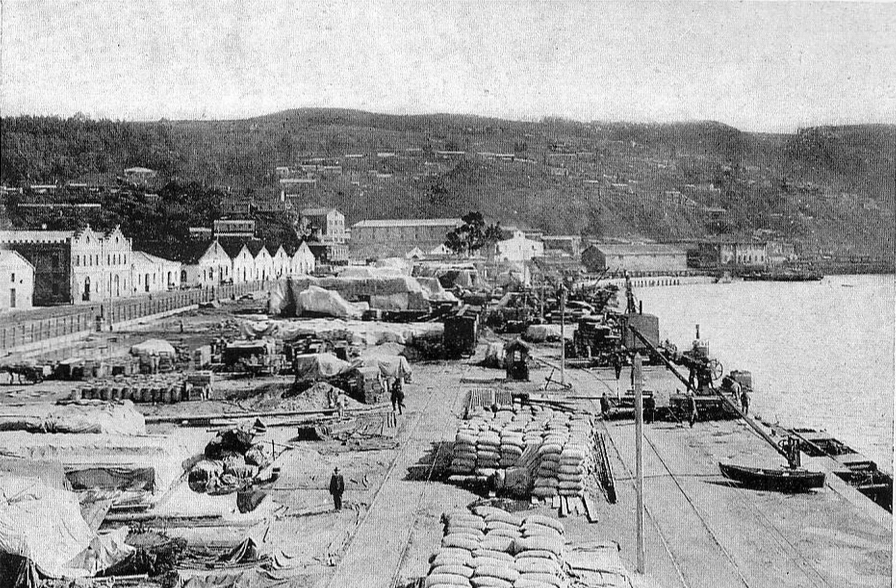
\includegraphics[scale=0.22]{/Users/hectorbahamonde/RU/Dissertation/Presentation/Resources/Talcahuano}}\caption*{{\tiny Talcahuano Port, Chile 19th Century.}}
		\label{fig:talcahuano}
		\end{figure}
	\end{columns}
\end{frame}
%%%%%%%%%%%%%%%%%%%%%%%%%%%%%%%%%%%%%%%%%%%%%%%%%%%%%%%%%%%%%%%%%%%%%%%%%%




%%%%%%%%%%%%%%%%%%%%%%%%%%%%%%%%%%%%%%%%%%%%%%%%%%%%%%%%%%%%%%%%%%%%%%%%%%
\defverbatim[colored]\lst{%
\begin{lstlisting}[tabsize=1,basicstyle=\TINY]
model.jags.sectoral <- function() {
for (i in 1:N){ # number of earthquakes

Deaths[i] ~ dpois(lambda[i]) log(lambda[i]) <- 
												b.propagrmanu[Sector[i]]*propagrmanu[i] + # multi-level
												b.Magnitude[Sector[i]]*Magnitude[i] + #  multi-level
												b.p.Population*p.Population[i] +
												b.Urban*Urban[i] +
												b.year[yearID[i]] + # year fixed-effects
												b.r.long*r.long[i] +
												b.r.lat*r.lat[i] +
												mu ## intercept
}

## Non-Informative/Flat Priors
b.r.lat ~ dnorm(0, 0.01)
b.r.long ~ dnorm(0, 0.01)
mu  ~ dnorm(0, 0.01) ## intercept
b.p.Population ~ dnorm(0, 0.01)
b.Urban ~ dnorm(0, 0.01)

## Year Fixed-Effects
for (t in 1:yearN){
					b.year[t] ~ dnorm(m.b.year[t], tau.b.year[t])
					m.b.year[t] ~ dnorm(0, 0.01)
					tau.b.year[t] ~ dgamma(0.5, 0.001) # uninformative Gamma priors
}
        
## Varying Slopes for Magnitude (unmodeled)
for (k in 1:NSector){# 
					b.Magnitude[k] ~ dnorm(m.Magnitude[k], tau.Magnitude[k])
					m.Magnitude[k] ~ dnorm(0, 0.01)
					tau.Magnitude[k] ~ dgamma(0.5, 0.001) # uninformative Gamma priors
					}

## Varying Slopes for Agr/Ind Proportion (unmodeled)
for (k in 1:NSector){# 
					b.propagrmanu[k] ~ dnorm(m.b.propagrmanu[k], tau.b.propagrmanu[k])
					m.b.propagrmanu[k] ~ dnorm(0, 0.01)
					tau.b.propagrmanu[k] ~ dgamma(0.5, 0.001) # uninformative Gamma priors
					}

	}

\end{lstlisting}
}

\begin{frame}[plain, label = jags_code]
\lst
\end{frame}

%%%%%%%%%%%%%%%%%%%%%%%%%%%%%%%%%%%%%%%%%%%%%%%%%%%%%%%%%%%%%%%%%%%%%%%%%%



%%%%%%%%%%%%%%%%%%%%%%%%%%%%%%%%%%%%%%%%%%%%%%%%%%%%%%%%%%%%%%%%%%%%%%%%%%
\begin{frame}[label=tax_sect_comp]\frametitle{Sectoral Competition and Taxation?}
Agricultural production, as it needs mostly land, it does not rely on capital as much as the industrial sector does. Moreover, they oppose taxation because their main asset (land) is fixed, hence landowners not being able to move their asset, resist taxation. On the contrary, industrial elites rely on public goods that are beneficial for their business (railroads, bridges, etc.). And while industrialists would prefer imposing higher import taxes (NOT the income tax), that increases the price of importing industrial capital (for ex., machines). Consequently, their second best choice is imposing an income tax.\\
For these reasons, the emergence of the industrial sector (which implies higher levels of sectoral/elite contestation) leads to the implementation of the income tax.
\end{frame}
%%%%%%%%%%%%%%%%%%%%%%%%%%%%%%%%%%%%%%%%%%%%%%%%%%%%%%%%%%%%%%%%%%%%%%%%%%



%%%%%%%%%%%%%%%%%%%%%%%%%%%%%%%%%%%%%%%%%%%%%%%%%%%%%%%%%%%%%%%%%%%%%%%%%%
\begin{frame}[label=origins_industry]\frametitle{Where does industry come from?}
{\bf p. 20 of dissertation}. Industry, as predicted by the dual sector model, came from agriculture: 
\tiny{

\begin{itemize}
\item After the mining boom, mining elites shifted their focus to what is considered the first \emph{true} industrial work which began under agricultural auspices: the cotton mills: ``[t]he first power looms were brought [in Per\'u, Ecuador, and Venezuela] in the 1840s, 1850s; but in all three they were a failure, some of the early mills in Ecuador being destroyed by an earthquake. It was not until after 1890 that the textile industries of these nations began to operate with reasonable success. Guatemala's first cotton mill was established in 1882, and between that date and 1910 a few mills appeared in Chile, Argentina, Uruguay, and Colombia.''\\

\item The first industries were called \emph{obrajes} and beyond textiles, early industrialists processed other agricultural goods. For example, animal grease and tallow, dried and cured meats, flour, bread, beer, wines and spirits, being most of them for domestic consumption. Sugar was used in the production of chocolate, candies and biscuits. 

\item The industrial sector was boosted by favorable international conditions, many times stimulating a positive complementarity between the two sectors. Industrial activities started very small, progressing ``from the shop to the factory during the latter half of the nineteenth century.'' 

\item Importantly, modern industrialization did \emph{not} begin with ISI, but around 1900. Others find that the ``fact that manufacturing was alive and thriving in Latin America before the 1929 crash is now beyond question.'' And that the ``development of large-scale, mechanized (and even ``heavy'') industry can be dated back to the 1890s.'' By the 1870's the carriage industry was on a firm basis.  
\end{itemize}

}

\end{frame}
%%%%%%%%%%%%%%%%%%%%%%%%%%%%%%%%%%%%%%%%%%%%%%%%%%%%%%%%%%%%%%%%%%%%%%%%%%


%%%%%%%%%%%%%%%%%%%%%%%%%%%%%%%%%%%%%%%%%%%%%%%%%%%%%%%%%%%%%%%%%%%%%%%%%%
\begin{frame}[label=death_count_plot]
 %\hspace{-1.16cm} 
 \centering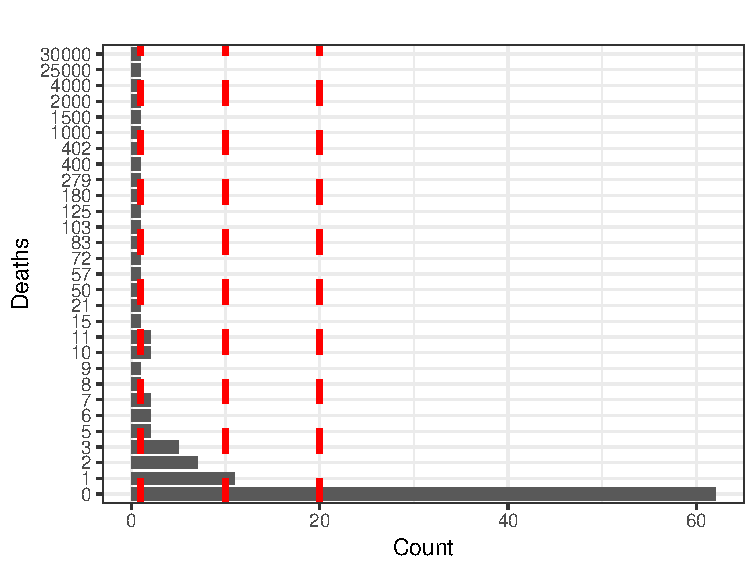
\includegraphics[scale=0.8]{/Users/hectorbahamonde/RU/Dissertation/Presentation/Resources/count_plot.pdf}
\end{frame}
%%%%%%%%%%%%%%%%%%%%%%%%%%%%%%%%%%%%%%%%%%%%%%%%%%%%%%%%%%%%%%%%%%%%%%%%%%



%%%%%%%%%%%%%%%%%%%%%%%%%%%%%%%%%%%%%%%%%%%%%%%%%%%%%%%%%%%%%%%%%%%%%%%%%%
\begin{frame}[label=where]\frametitle{But Where Does Industrialization Come From?!}

The theory puts heavy emphasis on the role of industrialization on state development. However, \emph{Where does industrialization come from?}
\\

Haber 2005 explains that:

``The impetus for industrial development came from the expansion of foreign trade. Driving the growth of foreign trade were two factors. The first was that most Latin American countries were on the silver standard, and silver fell in value relative to gold in the last two decades of the nineteenth century. Most Latin American countries therefore saw their currencies depreciate in real terms relative to the gold-backed currencies of the economies of the North Atlantic. As international trade theory would predict, real exchange rate depreciation resulted in the expansion of the tradables (e.g. industrial goods) [...] Second, the late nineteenth century also saw a dramatic decline in the international costs of transport, as steel-hulled steamships came to replace wood and sail.''

\end{frame}
%%%%%%%%%%%%%%%%%%%%%%%%%%%%%%%%%%%%%%%%%%%%%%%%%%%%%%%%%%%%%%%%%%%%%%%%%%




%%%%%%%%%%%%%%%%%%%%%%%%%%%%%%%%%%%%%%%%%%%%%%%%%%%%%%%%%%%%%%%%%%%%%%%%%%
\begin{frame}[label=conflict]\frametitle{From Conflict to Cooperation}

Why do lower levels of {\bf sectoral inequality} (which implied {\bf higher military threats}) lead to {\bf sectoral cooperation}?

The rising of the industrial sector allowed industrial political elites to get access to military capacities that were as good as the agricultural elite's. The {\bf threat} is what leads to {\bf cooperation} rather than {\bf conflict}. It makes no sense to engage in conflict when (1) both groups have the same `fire power' and (2) when there is a cheaper exit (sectoral bargains).

\end{frame}
%%%%%%%%%%%%%%%%%%%%%%%%%%%%%%%%%%%%%%%%%%%%%%%%%%%%%%%%%%%%%%%%%%%%%%%%%%





%%%%%%%%%%%%%%%%%%%%%%%%%%%%%%%%%%%%%%%%%%%%%%%%%%%%%%%%%%%%%%%%%%%%%%%%%%
\begin{frame}[label=1891_1924]\frametitle{War was in 1891, but Income Tax in 1924?}
\begin{itemize} \tiny
	\item Civil wars of {\bf 1851-859} and {\bf 1891} between a ``{\bf large landed property [elite against a] productive capital [elite]}.''

	\item President {\bf Balmaceda's overthrowing in 1891} explains the sectoral nature of these conflicts. 

	\item He was mainly supported by the landed elites, but later overthrown in 1891 by a mainly industrial/mining coalition:

		\begin{itemize} \tiny

			\item His agenda on ``industrial'' infrastructure benefited mostly agricultural areas.

			\item his attitude towards the banking sector (closely linked to the mining sector) confiscatory.

		\end{itemize}


	\item At the same time, however, he failed to secure a coalition with his own sector. 

	\begin{itemize} \tiny
		\item Decline of wheat exports. Balmaceda's policies fostered sectoral dependence of agriculture on industrial production, forcing the ``landed proprietors [to] become dependent to a considerable extent on the continuing prosperity of the major nitrate capitalists.'' (Zeitlin).

		\item While it would be inaccurate to say that Balmaceda was \emph{completely} supported by agriculturalists and \emph{completely} opposed by industrialists, this example illustrates how (failed) inter-sectoral alliances and biased public goods provision against industrialists led these two groups to a military conflict in 1891. 

		\item The conflict left a permanent scar in the Chilean society. While the civil war lasted only nine months, it took 10,000 lives (out of a total population of 3 million people) and cost more than \$ 100 million,a significant amount for a small country. 

		\item There was an intention to avoid more violence. For instance, while all ``ministers, counselors of state, members of the constituent congress [,] municipal officials, provincial governors and intendants, members of the judiciary and even the lowest functionaries and ordinary employees of Balmaceda's government were investigated [or] brought to trial,'' there were a number of amnesties issued. Similarly, there were a number of \emph{aborted} coups in 1907, 1912, 1915 and 1919. I identify a third additional factor. War was more likely to exhaust all existent assets without producing positive outcomes for either sector, putting pressures for a sectoral compromise.
	\end{itemize}

\end{itemize}

\end{frame}
%%%%%%%%%%%%%%%%%%%%%%%%%%%%%%%%%%%%%%%%%%%%%%%%%%%%%%%%%%%%%%%%%%%%%%%%%%





%%%%%%%%%%%%%%%%%%%%%%%%%%%%%%%%%%%%%%%%%%%%%%%%%%%%%%%%%%%%%%%%%%%%%%%%%%
% unit roots
\begin{frame}[label=unit_root]
\scalebox{0.2}{

\begin{tabular}{ c c c c c c c } 
{\bf Country} & Time Frame & {\bf Sector} & {\bf Augmented Dickey-Fuller}  & {\bf Phillips-Perron} & {\bf KPSS} & {\bf Conclusion} \\
\\\multirow{6}{*}{Chile}& \multirow{2}{*}{Pre}  & Agriculture & -1.185 (0.68) & -1.241 (0.66)   & .107$^{\dagger}$ &  I(1)\\
\\                        &                         & Industry    & 2.310 (0.99) & 2.556 (0.99) & .113$^{\dagger}$ &  I(1)\\
\\                        & \multirow{2}{*}{Post} & Agriculture & 4.557 (1.00) & 5.40 (1.00)    & .289 &  I(1)\\
\\                        &                         & Industry    & 0.908 (0.99) & 1.458 (0.99) & .249 &  I(1)\\                      
\\                        & \multirow{2}{*}{All}  & Agriculture & 5.521 (1.00) & 6.722 (1.00)   & .31  &  I(1)\\
\\                        &                         & Industry    & 1.582 (0.99) & 2.305 (0.99) & .314 &  I(1)\\
\\\multirow{6}{*}{Colombia}& \multirow{2}{*}{Pre}  & Agriculture & 2.709 (0.99) & 2.414 (0.99)  & .204 &  I(1)\\
\\                        &                         & Industry    &  2.103 (0.99) & 3.257 (1.00)& .183 &  I(1)\\
\\                        & \multirow{2}{*}{Post} & Agriculture & 2.392 (0.99) & 3.156 (1.00)   & .282 &  I(1)\\
\\                        &                         & Industry    & 0.520 (0.98) & 1.044 (0.99) & .241 &  I(1)\\                       
\\                        & \multirow{2}{*}{All}  & Agriculture & 4.256 (1.00) & 5.893 (1.00)   & .372 &  I(1)\\
\\                        &                         & Industry    & 1.674 (0.99) & 2.707 (0.99) & .374 &  I(1)\\
\\\multirow{6}{*}{Argentina}& \multirow{2}{*}{Pre}  & Agriculture & -0.849 (0.80) & -1.201 (0.67) & .0801$^{\dagger}$ &  I(1)\\
\\                        &                         & Industry    & -0.495 (0.89) & -0.378 (0.91) & .115$^{\dagger}$ &  I(1)\\
\\                        & \multirow{2}{*}{Post} & Agriculture & 1.197 (0.99) & 1.093 (0.99) & .277 &  I(1)\\
\\                        &                         & Industry    & 0.228 (0.97) & 0.381 (0.98) & .0901$^{\dagger}$ & I(1)\\                  
\\                        & \multirow{2}{*}{All}  & Agriculture & 1.484 (0.99)  & 1.401 (0.99) & .332 & I(1)\\
\\                        &                         & Industry    & 1.007 (0.99) & 1.237 (0.99) & .183 & I(1)\\
\\\multirow{6}{*}{Mexico}& \multirow{2}{*}{Pre}  & Agriculture & 4.601 (1.00) & 5.552 (1.00) & .288 & I(1)\\
\\                        &                         & Industry & 5.803 (1.00) & 10.776 (1.00) & .29 & I(1)\\  
\\                        & \multirow{2}{*}{Post} & Agriculture & 0.599 (0.9876) & 0.497 (0.99) & .109$^{\dagger}$ & I(1)\\
\\                        &                         & Industry   & -1.255 (0.65) & -0.982 (0.76) & .113$^{\dagger}$ & I(1)\\                        
\\                        & \multirow{2}{*}{All}  & Agriculture & 3.431 (1.00) & 3.607 (1.00) & .341 & I(1)\\
\\                        &                         & Industry  & 0.672 (0.99) & 2.020 (0.99) & .367 & I(1)\\
\\\multirow{6}{*}{Nicaragua}& \multirow{2}{*}{Pre}  & Agriculture & 2.473 (0.99) & 2.355 (0.99) & .25 & I(1)\\
\\                        &                         & Industry    & 4.958 (1.00) & 9.100 (1.00) & .244 & I(1)\\  
\\                        & \multirow{2}{*}{Post} & Agriculture & -0.154 (0.94) & 0.154 (0.97) & .2 & I(1)\\
\\                        &                         & Industry    & -1.237 (0.6577) & -1.176 (0.68) & .189 & I(1)\\                        
\\                        & \multirow{2}{*}{All}    & Agriculture & 0.636 (0.99) & 0.759 (0.99) & .116$^{\dagger}$ & I(1)\\
\\                        &                         & Industry    & -0.164 (0.94) & -0.090 (0.95) & .123 & I(1)\\
\\\multirow{6}{*}{Guatemala}& \multirow{2}{*}{Pre}  & Agriculture & -0.393 (0.91) & -0.343 (0.92) & .0639$^{\dagger}$ & I(1)\\
\\                        &                         & Industry    & 1.358 (0.99)  & 1.704 (0.99) & .199 & I(1)\\  
\\                        & \multirow{2}{*}{Post} & Agriculture & 1.786 (0.99)  & 1.965 (0.99) & .162 & I(1)\\
\\                        &                       & Industry    & -0.998 (0.75) & -1.352 (0.61) & .0915$^{\dagger}$ & I(1)\\                        
\\                        & \multirow{2}{*}{All}  & Agriculture & 3.349 (1.00) & 3.714 (1.00) & .321 & I(1)\\
\\                        &                       & Industry    & 0.413 (0.98) & 0.017 (0.96) & .288 & I(1)\\
\end{tabular}
}
\end{frame}
%%%%%%%%%%%%%%%%%%%%%%%%%%%%%%%%%%%%%%%%%%%%%%%%%%%%%%%%%%%%%%%%%%%%%%%%%%





%%%%%%%%%%%%%%%%%%%%%%%%%%%%%%%%%%%%%%%%%%%%%%%%%%%%%%%%%%%%%%%%%%%%%%%%%%
% cointegration tests
\begin{frame}[label=johansen_tests]

\scalebox{0.6}{

\begin{tabular}{ c | c  c c c c }
{\bf Country} & {\bf Number of Cointegrated Vectors (rank)} &  Restrictions & {\bf Lags} & {\bf Log-Likelihood} & {\bf Trace} \\[-.1em] 
\hline
Chile       & at least 1 & Restricted Constant  & 5 & -1665.9736 & 0.3799\\[.2em] 
Argentina   & at least 1 & Restricted Constant  & 3 & -1802.292 & 4.7657\\[.2em] 
Colombia    & at least 1 & Restricted Trend  	& 2 & -1805.6773 & 10.0076\\[.2em] 
Mexico      & at least 1 & Restricted Constant  & 4 & -1978.1322 & 1.0274\\[.2em] 
Nicaragua   & 0 & Restricted Constant 	& 2 & -1020.221 & 11.5297 \\[.2em] 
Guatemala   & 0 & Trend 				& 3 & -859.2802 & 16.5493 \\[.2em] 
\end{tabular} 
}
\end{frame}
%%%%%%%%%%%%%%%%%%%%%%%%%%%%%%%%%%%%%%%%%%%%%%%%%%%%%%%%%%%%%%%%%%%%%%%%%%

% defines a checkmark and x mark symbols
\newcommand{\cmark}{\ding{51}}%
\newcommand{\xmark}{\ding{55}}%






%%%%%%%%%%%%%%%%%%%%%%%%%%%%%%%%%%%%%%%%%%%%%%%%%%%%%%%%%%%%%%%%%%%%%%%%%%
% lags
\begin{frame}[label=lags_tests]

\scalebox{0.5}{

%% Lag Length and Post-Estimation Results // post:estimation:lag:lenght:tests

\begin{tabular}{ c c | c c c c c c } 
{\bf Country} & {\bf Time Frame} & {\bf Number of Lags} & {\bf LM} & \multicolumn{3}{c}{{\bf Normally Tests}}  & {\bf Stability Condition}\\
              &                  &                      &          & \emph{Jarque-Bera} &  \emph{Skewness} &  \emph{Kurtosis}    & \\
\hline
\\\multirow{2}{*}{Chile}  & Pre   & 4 & \cmark & \cmark & \cmark & \cmark & \cmark \\
\\                        & Post  & 2 & \cmark & \cmark$^{-}$ & \cmark$^{-}$ & \cmark$^{-}$ & \cmark \\[.2em]\cline{3-8}
\\\multirow{2}{*}{Colombia}   & Pre   & 1 & \cmark$^{-}$ & \xmark & \xmark & \xmark & \cmark \\
\\                            & Post  & 1 & \cmark & \cmark$^{-}$ & \cmark$^{-}$ & \cmark$^{-}$ & \cmark \\[.2em]\cline{3-8}
\\\multirow{2}{*}{Argentina}  & Pre   & 2 & \cmark & \cmark & \cmark & \cmark & \cmark \\
\\                            & Post  & 2 & \cmark & \cmark$^{-}$ & \cmark & \cmark$^{-}$ & \cmark \\[.2em]\cline{3-8}
\\\multirow{2}{*}{Mexico} & Pre   & 1 & \cmark & \cmark$^{-}$ & \cmark$^{-}$ & \cmark$^{-}$ & \cmark \\
\\                        & Post  & 2 & \cmark & \cmark & \cmark & \cmark & \cmark \\[.2em]\cline{3-8}
\\\multirow{2}{*}{Nicaragua}  & Pre   & 2 & \cmark & \cmark$^{-}$ & \cmark$^{-}$ & \cmark$^{-}$ & \cmark \\
\\                            & Post  & 1 & \cmark & \cmark$^{-}$ & \cmark$^{-}$ & \cmark$^{-}$ & \cmark \\[.2em]\cline{3-8}
\\\multirow{2}{*}{Guatemala}  & Pre   & 3 & \cmark & \xmark & \cmark$^{-}$ & \cmark$^{-}$ & \cmark \\
\\                            & Post  & 1 & \cmark$^{-}$ & \cmark$^{-}$ & \cmark$^{-}$ & \cmark$^{-}$ & \cmark \\
\end{tabular}
}

\end{frame}
%%%%%%%%%%%%%%%%%%%%%%%%%%%%%%%%%%%%%%%%%%%%%%%%%%%%%%%%%%%%%%%%%%%%%%%%%%





%%%%%%%%%%%%%%%%%%%%%%%%%%%%%%%%%%%%%%%%%%%%%%%%%%%%%%%%%%%%%%%%%%%%%%%%%%
% ts_plots
% All countries Sectoral Outputs
\begin{frame}[label=ts_plots]
 %\hspace{-1.16cm} 
 \centering\includegraphics[scale=0.75]{/Users/hectorbahamonde/RU/Dissertation/Papers/NegativeLink/Structural_Breaks_Paper.pdf}
\end{frame}
%%%%%%%%%%%%%%%%%%%%%%%%%%%%%%%%%%%%%%%%%%%%%%%%%%%%%%%%%%%%%%%%%%%%%%%%%%




%%%%%%%%%%%%%%%%%%%%%%%%%%%%%%%%%%%%%%%%%%%%%%%%%%%%%%%%%%%%%%%%%%%%%%%%%%
% granger_tests
\begin{frame}[label=granger_test]
\scalebox{0.3}{

\begin{tabular}{ c c c c c c } 
{\bf Country} & {\bf Pre/Post Income Tax } & {\bf Sample} & {\bf Directionality} & {\bf chi2}  & {\bf P-value} \\
\\\multirow{4}{*}{Chile} & \multirow{2}{*}{Pre}  & \multirow{2}{*}{1905 - 1924} & Agriculture $\rightarrow$ Industry & 3.55 & 0.47\\
\\                       &                       &                              & Industry $\rightarrow$ Agriculture & 12.13 & 0.02 \\ [.2em]\cline{2-6}
\\                       & \multirow{2}{*}{Post} & \multirow{2}{*}{1928 - 2009} & Agriculture $\rightarrow$ Industry & 11.92 & 0.00 \\
\\                       &                       &                              & Industry $\rightarrow$ Agriculture & 5.37 & 0.07 \\
\hline
\\\multirow{4}{*}{Colombia} & \multirow{2}{*}{Pre}  & \multirow{2}{*}{1902 - 1935} & Agriculture $\rightarrow$ Industry & 4.96 & 0.03 \\
\\                          &                       &                              & Industry $\rightarrow$ Agriculture & 10.44 & 0.00 \\ [.2em]\cline{2-6}
\\                          & \multirow{2}{*}{Post} & \multirow{2}{*}{1938 - 2009} & Agriculture $\rightarrow$ Industry & 4.32 & 0.04 \\
\\                          &                       &                              & Industry $\rightarrow$ Agriculture & 1.63 & 0.20 \\
\hline
\\\multirow{4}{*}{Argentina}  & \multirow{2}{*}{Pre}  & \multirow{2}{*}{1903 - 1933}  & Agriculture $\rightarrow$ Industry & 4.19 & 0.12 \\
\\                            &                       &                               & Industry $\rightarrow$ Agriculture & .42 & 0.81 \\ [.2em]\cline{2-6}
\\                            & \multirow{2}{*}{Post} & \multirow{2}{*}{1937 - 2010}  & Agriculture $\rightarrow$ Industry & .18 & 0.91 \\
\\                            &                       &                               & Industry $\rightarrow$ Agriculture & 1.37 & 0.50 \\
\hline
\\\multirow{4}{*}{Mexico} & \multirow{2}{*}{Pre}  & \multirow{2}{*}{1902 - 1965}  & Agriculture $\rightarrow$ Industry & .73 & 0.39 \\
\\                        &                       &                               & Industry $\rightarrow$ Agriculture & 11.57 & 0.00 \\ [.2em]\cline{2-6}
\\                        & \multirow{2}{*}{Post} & \multirow{2}{*}{1969 - 2009}  & Agriculture $\rightarrow$ Industry & 5.56  & 0.06 \\
\\                        &                       &                               & Industry $\rightarrow$ Agriculture & 1.32 &  0.52 \\
\hline
\\\multirow{4}{*}{Nicaragua}  & \multirow{2}{*}{Pre}  & \multirow{2}{*}{1923 - 1974}  & Agriculture $\rightarrow$ Industry & .48 & 0.79 \\
\\                            &                       &                               & Industry $\rightarrow$ Agriculture & 6.83 & 0.03 \\ [.2em]\cline{2-6}
\\                       & \multirow{2}{*}{Post}      & \multirow{2}{*}{1977 - 2009}  & Agriculture $\rightarrow$ Industry & .014 & 0.91 \\
\\                       &                            &                               & Industry $\rightarrow$ Agriculture & 4.96 & 0.03 \\
\hline
\\\multirow{4}{*}{Guatemala}  & \multirow{2}{*}{Pre} & \multirow{2}{*}{1924 - 1963} & Agriculture $\rightarrow$ Industry & 2.18 & 0.54 \\
\\                            &                      &                              & Industry $\rightarrow$ Agriculture & 6.72 & 0.08 \\ [.2em]\cline{2-6}
\\                            & \multirow{2}{*}{Post}& \multirow{2}{*}{1966 - 2009} & Agriculture $\rightarrow$ Industry & .58 & 0.45 \\
\\                            &                      &                              & Industry $\rightarrow$ Agriculture &  6.05 & 0.01 \\
\end{tabular}

}
\end{frame}
%%%%%%%%%%%%%%%%%%%%%%%%%%%%%%%%%%%%%%%%%%%%%%%%%%%%%%%%%%%%%%%%%%%%%%%%%%




%%%%%%%%%%%%%%%%%%%%%%%%%%%%%%%%%%%%%%%%%%%%%%%%%%%%%%%%%%%%%%%%%%%%%%%%%%
% sectoral plots: Densities
\begin{frame}[label=density_plot_sectoral]
 \centering\includegraphics[scale=0.3]{/Users/hectorbahamonde/RU/Dissertation/Papers/Earthquake_Paper/figure/denplot:plot:sectoral-1.pdf}
\end{frame}
%%%%%%%%%%%%%%%%%%%%%%%%%%%%%%%%%%%%%%%%%%%%%%%%%%%%%%%%%%%%%%%%%%%%%%%%%%




%%%%%%%%%%%%%%%%%%%%%%%%%%%%%%%%%%%%%%%%%%%%%%%%%%%%%%%%%%%%%%%%%%%%%%%%%%
% sectoral plots: Trace plots
\begin{frame}[label=trace_plot_sectoral]
%\hspace{-1.16cm} 
\centering\includegraphics[scale=0.3]{/Users/hectorbahamonde/RU/Dissertation/Papers/Earthquake_Paper/figure/traplot:plot:sectoral-1}
\end{frame}
%%%%%%%%%%%%%%%%%%%%%%%%%%%%%%%%%%%%%%%%%%%%%%%%%%%%%%%%%%%%%%%%%%%%%%%%%%





%%%%%%%%%%%%%%%%%%%%%%%%%%%%%%%%%%%%%%%%%%%%%%%%%%%%%%%%%%%%%%%%%%%%%%%%%%
% sectoral and tax plot: Model Fit of Both models
\begin{frame}[label=model_fit]
%\hspace{-1.16cm} 
\centering\includegraphics[scale=0.3]{/Users/hectorbahamonde/RU/Dissertation/Papers/Earthquake_Paper/figure/predicted:observed:plot-1}
\end{frame}
%%%%%%%%%%%%%%%%%%%%%%%%%%%%%%%%%%%%%%%%%%%%%%%%%%%%%%%%%%%%%%%%%%%%%%%%%%




%%%%%%%%%%%%%%%%%%%%%%%%%%%%%%%%%%%%%%%%%%%%%%%%%%%%%%%%%%%%%%%%%%%%%%%%%%
% sectoral model: dependent variable
\begin{frame}[label=proportion_variable]
%\hspace{-1.16cm} 
\centering\includegraphics[scale=0.7]{/Users/hectorbahamonde/RU/Dissertation/Papers/Earthquake_Paper/figure/incometax-1}
\end{frame}
%%%%%%%%%%%%%%%%%%%%%%%%%%%%%%%%%%%%%%%%%%%%%%%%%%%%%%%%%%%%%%%%%%%%%%%%%%




%%%%%%%%%%%%%%%%%%%%%%%%%%%%%%%%%%%%%%%%%%%%%%%%%%%%%%%%%%%%%%%%%%%%%%%%%%
% sectoral model: Reg. Table
\begin{frame}[label=table_sectoral]
\begin{tabular}{rrrrrr}
  \hline
 & Mean & SD & Lower & Upper & Pr. \\ 
  \hline
Agr/Ind [Agr] & 12.68 & 7.21 & 3.73 & 22.65 & 0.98 \\ 
  Agr/Ind [Ind] & -16.26 & 5.30 & -23.17 & -9.62 & 1.00 \\ 
  Agr/Ind [Mixed] & -30.73 & 21.74 & -63.78 & -4.89 & 0.95 \\ 
  Magnitude [Agr] & 0.04 & 0.02 & 0.01 & 0.06 & 0.95 \\ 
  Magnitude [Ind] & 0.24 & 0.07 & 0.16 & 0.32 & 1.00 \\ 
  Magnitude [Mixed] & 0.37 & 0.14 & 0.17 & 0.55 & 1.00 \\ 
  Latitude & -0.01 & 0.03 & -0.05 & 0.02 & 0.69 \\ 
  Longitude & -0.16 & 0.14 & -0.34 & 0.03 & 0.85 \\ 
  Population & -0.01 & 0.00 & -0.02 & -0.01 & 1.00 \\ 
  Urban & -1.54 & 2.01 & -4.22 & 1.00 & 0.76 \\ 
   \hline 
 \multicolumn{6}{c}{ \scriptsize {\bf Note}: 200000 iterations with a burn-in period of n = 5000 iterations discarded.}\\
 \multicolumn{6}{c}{ \scriptsize 80\% credible intervals (upper/lower bounds). All R-Hat statistics below critical levels.}\\
 \multicolumn{6}{c}{ \scriptsize Standard convergence diagnostics suggest good mixing and convergence.}\\
 \multicolumn{6}{c}{ \scriptsize Year fixed effects were omitted in the table.}
 \\\end{tabular}
\end{frame}
%%%%%%%%%%%%%%%%%%%%%%%%%%%%%%%%%%%%%%%%%%%%%%%%%%%%%%%%%%%%%%%%%%%%%%%%%%







%%%%%%%%%%%%%%%%%%%%%%%%%%%%%%%%%%%%%%%%%%%%%%%%%%%%%%%%%%%%%%%%%%%%%%%%%%
% tax plots: Densities
\begin{frame}[label=density_plot_tax]
 \centering\includegraphics[scale=0.35]{/Users/hectorbahamonde/RU/Dissertation/Papers/Earthquake_Paper/figure/denplot:plot:tax-1.pdf}
\end{frame}
%%%%%%%%%%%%%%%%%%%%%%%%%%%%%%%%%%%%%%%%%%%%%%%%%%%%%%%%%%%%%%%%%%%%%%%%%%





%%%%%%%%%%%%%%%%%%%%%%%%%%%%%%%%%%%%%%%%%%%%%%%%%%%%%%%%%%%%%%%%%%%%%%%%%%
% tax plots: Trace plots
\begin{frame}[label=trace_plot_tax]
%\hspace{-1.16cm} 
\centering\includegraphics[scale=0.35]{/Users/hectorbahamonde/RU/Dissertation/Papers/Earthquake_Paper/figure/traplot:plot:tax-1}
\end{frame}
%%%%%%%%%%%%%%%%%%%%%%%%%%%%%%%%%%%%%%%%%%%%%%%%%%%%%%%%%%%%%%%%%%%%%%%%%%








%%%%%%%%%%%%%%%%%%%%%%%%%%%%%%%%%%%%%%%%%%%%%%%%%%%%%%%%%%%%%%%%%%%%%%%%%%
% tax model: Reg. Table
\begin{frame}[label=table_tax]
\begin{tabular}{rrrrrr}
  \hline
 & Mean & SD & Lower & Upper & Pr. \\ 
  \hline
Income Tax & -3.01 & 3.55 & -7.55 & 1.41 & 0.81 \\ 
  Magnitude & 0.06 & 0.01 & 0.04 & 0.07 & 1.00 \\ 
  Latitude & 0.06 & 0.01 & 0.04 & 0.08 & 1.00 \\ 
  Longitude & -0.49 & 0.07 & -0.58 & -0.39 & 1.00 \\ 
  Population & -0.02 & 0.00 & -0.02 & -0.02 & 1.00 \\ 
  Urban & -5.22 & 0.73 & -6.19 & -4.35 & 1.00 \\ 
   \hline 
 \multicolumn{6}{l}{ \scriptsize {\bf Note}: 200000 iterations with a burn-in period of n = 5000 iterations discarded.}\\
 \multicolumn{6}{l}{ \scriptsize 80\% credible intervals (upper/lower bounds). All R-Hat statistics below critical levels.}\\
 \multicolumn{6}{l}{ \scriptsize Standard convergence diagnostics suggest good mixing and convergence.}\\
 \multicolumn{6}{l}{ \scriptsize Year fixed effects were omitted in the table.}\\
 \multicolumn{6}{l}{ \scriptsize A total of 4 chains were run. Detailed diagnostic plots available \href{https://github.com/hbahamonde/Earthquake_Paper/raw/master/Bahamonde_Earthquake_Paper_Diagnostic_Plots_Income_Tax_Model.pdf}{\texttt here}.}
 \end{tabular}
\end{frame}
%%%%%%%%%%%%%%%%%%%%%%%%%%%%%%%%%%%%%%%%%%%%%%%%%%%%%%%%%%%%%%%%%%%%%%%%%%



%%%%%%%%%%%%%%%%%%%%%%%%%%%%%%%%%%%%%%%%%%%%%%%%%%%%%%%%%%%%%%%%%%%%%%%%%%
\begin{frame}[label=credible_threats]
For example, the historian Barros (1970) explains that before the civil war, \emph{salitreras} (nitrate towns) in northern Chile were locally so important that they were considered ``a state within the state.'' {\bf Local bosses had to approve decisions on whether public employees could be fired, whether public works could be developed, and on whether politicians could give public speeches}. Moreover, {\color{red}they coined their own currency} and had their own particular {\color{red}local laws}. 
\end{frame}
%%%%%%%%%%%%%%%%%%%%%%%%%%%%%%%%%%%%%%%%%%%%%%%%%%%%%%%%%%%%%%%%%%%%%%%%%%




\begin{frame}[plain,c, label=thank_you]


\begin{center}
\Huge{Thank you!}\\
\vspace{1cm} - \large{{\bf Download Papers}: \texttt{www.Hector{\color{black!30!green}{\bf Bahamonde}}.com/research/}\\
\vspace{1cm} - {\bf Code/Data}: GitHub \texttt{h{\color{black!30!green}{\bf bahamonde}}}}\\
\vspace{1cm} - {\bf More info}: \texttt{www.Hector{\color{black!30!green}{\bf Bahamonde}}.com}
\end{center}

\vspace{1cm}
% \hspace{5cm}
\centering\scalebox{0.7}{\hyperlink{toc}{\beamerbutton{TOC}}}
%\vspace{2cm}\hspace{5cm}
\centering\scalebox{0.7}{\hyperlink{cover}{\beamerbutton{Cover}}}
\end{frame}



\end{document}


%\begin{align*}
%ATE 	=& E[\tau | \vec{X}]\\
%	=& \frac{1}{n}\sum\limits_{i=0}^n E[Y_{i}\text{(Treated)} - Y_{i}\text{(Untreated)} | \vec{X}]
%\end{align*}


% independence symbol \independent
%\newcommand\independent{\protect\mathpalette{\protect\independenT}{\perp}}
%\def\independenT#1#2{\mathrel{\rlap{$#1#2$}\mkern2mu{#1#2}}}


%\begin{equation*}
%i_{T} = i^{\prime}_{C} | \vec{X_{10}}
%\end{equation*}

%\begin{frame}
%\centering
%\only<1->{\includegraphics[width=6cm]{distributions1.pdf}}
%\end{frame}

%\begin{frame}
%\begin{columns}

%\column{0.4\textwidth}
%\begin{block}<1->{Defining Clientelism}
% Clientelism is a ``{\bf direct} [and {\bf contingent}] exchange of a citizen$'$s vote in return for direct payments or continuing access to employment, [private] goods, and services''
%\end{block}
%\column{0.6\textwidth}
%\begin{figure}[H]
%\includegraphics[scale=0.32, center]{pic3.jpg}
%\end{figure}
%\end{columns}
%\end{frame}
